
\documentclass[a4paper,UKenglish,cleveref, autoref, thm-restate]{lipics_v2021}
%This is a template for producing LIPIcs articles. 
%See lipics-v2021-authors-guidelines.pdf for further information.
%for A4 paper format use option "a4paper", for US-letter use option "letterpaper"
%for british hyphenation rules use option "UKenglish", for american hyphenation rules use option "USenglish"
%for section-numbered lemmas etc., use "numberwithinsect"
%for enabling cleveref support, use "cleveref"
%for enabling autoref support, use "autoref"
%for anonymousing the authors (e.g. for double-blind review), add "anonymous"
%for enabling thm-restate support, use "thm-restate"
%for enabling a two-column layout for the author/affilation part (only applicable for > 6 authors), use "authorcolumns"
%for producing a PDF according the PDF/A standard, add "pdfa"

\pdfoutput=1 %uncomment to ensure pdflatex processing (mandatatory e.g. to submit to arXiv)
\hideLIPIcs  %uncomment to remove references to LIPIcs series (logo, DOI, ...), e.g. when preparing a pre-final version to be uploaded to arXiv or another public repository

%\graphicspath{{./graphics/}}%helpful if your graphic files are in another directory

\bibliographystyle{plainurl}% the mandatory bibstyle

\title{Improved Approximations for Translational Packing of Convex Polygons} %TODO Please add

%\titlerunning{Dummy short title} %TODO optional, please use if title is longer than one line

\author{Adam Kurpisz}{Bern University of Applied Sciences and Department of Mathematics, ETH Zurich, Switzerland \and \url{https://n.ethz.ch/~kurpisza/} }{adam.kurpisz@ifor.math.ethz.ch}{https://orcid.org/0000-0002-2320-4482}{}%TODO mandatory, please use full name; only 1 author per \author macro; first two parameters are mandatory, other parameters can be empty. Please provide at least the name of the affiliation and the country. The full address is optional. Use additional curly braces to indicate the correct name splitting when the last name consists of multiple name parts.

\author{Silvan Suter}{Department of Mathematics, ETH Zurich, Switzerland}{sili.suter@bluewin.ch}{[orcid]}{}

\authorrunning{A. Kurpisz and S. Suter} %TODO mandatory. First: Use abbreviated first/middle names. Second (only in severe cases): Use first author plus 'et al.'

\Copyright{Adam Kurpisz and Silvan Suter} %TODO mandatory, please use full first names. LIPIcs license is "CC-BY";  http://creativecommons.org/licenses/by/3.0/


\ccsdesc[500]{Theory of computation~Packing and covering problems}
%\ccsdesc[100]{\textcolor{red}{Replace ccsdesc macro with valid one}} %TODO mandatory: Please choose ACM 2012 classifications from https://dl.acm.org/ccs/ccs_flat.cfm 

\keywords{Approximation algorithms, Packing problems, Convex polygons, Bin packing, Strip packing, Area minimization} %TODO mandatory; please add comma-separated list of keywords

\category{} %optional, e.g. invited paper

\relatedversion{This is the full version of the same-named ESA 2023 paper. A link will be provided in a future version of this document.} %optional, e.g. full version hosted on arXiv, HAL, or other respository/website
%\relatedversiondetails[linktext={arXiv}]{Extended Version}{www.arxiv.org} %linktext and cite are optional

%\supplement{}%optional, e.g. related research data, source code, ... hosted on a repository like zenodo, figshare, GitHub, ...
%\supplementdetails[linktext={opt. text shown instead of the URL}, cite=DBLP:books/mk/GrayR93, subcategory={Description, Subcategory}, swhid={Software Heritage Identifier}]{General Classification (e.g. Software, Dataset, Model, ...)}{URL to related version} %linktext, cite, and subcategory are optional

%\funding{(Optional) general funding statement \dots}%optional, to capture a funding statement, which applies to all authors. Please enter author specific funding statements as fifth argument of the \author macro.

%\acknowledgements{I want to thank \dots}%optional

\nolinenumbers %uncomment to disable line numbering


%all these lines added from me
\newtheorem{problem}[theorem]{Problem}
% \usepackage{amsthm}

% \makeatletter
% \newtheorem*{rep@theorem}{\rep@title}
% \newcommand{\newreptheorem}[2]{%
% \newenvironment{rep#1}[1]{%
%  \def\rep@title{#2 \ref{##1}}%
%  \begin{rep@theorem}}%
%  {\end{rep@theorem}}}
% %\newcommand{\newreptheorem}[2]{\newtheorem*{rep@#1}{\rep@title}\newenvironment{rep#1}[1]{\def\rep@title{#2 \ref*{##1}}\begin{rep@#1}}{\end{rep@#1}}}
% \makeatother

% \newreptheorem{theorem}{Theorem}

\usepackage{thmtools}
\usepackage{thm-restate}

\DeclareMathOperator{\sgn}{sgn}
\DeclareMathOperator{\dist}{dist}
\DeclareMathOperator{\opt}{opt}
\DeclareMathOperator{\cat}{\widetilde{\ca}}
\DeclareMathOperator{\pog}{PoG}
\DeclareMathOperator{\apog}{APoG}
\DeclareMathOperator{\argmin}{argmin}
\DeclareMathOperator{\argmax}{argmax}
\DeclareMathOperator{\Rectim}{\hspace{0.05 cm} 
\includegraphics[scale=0.02]{Images/rectangle_im3}}
\DeclareMathOperator{\rectangles}{\mathcal{I}_{\Rectim}}
\DeclareMathOperator{\Polyim}{\hspace{0.02 cm} 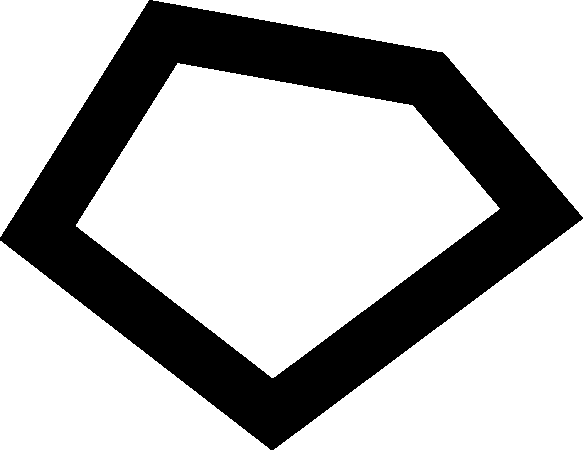
\includegraphics[scale=0.03]{Images/polygon_im3}}
\DeclareMathOperator{\polygons}{\mathcal{I}_{\Polyim}}
\DeclareMathOperator{\area}{\mathtt{area}}
\DeclareMathOperator{\width}{\mathtt{width}}
\DeclareMathOperator{\height}{\mathtt{height}}
\DeclareMathOperator{\base}{\mathtt{base}}
\DeclareMathOperator{\wside}{\mathtt{wside}}
\DeclareMathOperator{\conv}{conv}
\DeclareMathOperator{\interior}{int}
\DeclareMathOperator{\closure}{clos}
\DeclareMathOperator{\relint}{relint}
\DeclareMathOperator{\vertices}{vertices}
\DeclareMathOperator{\poly}{poly}
\DeclareMathOperator{\R}{\mathbb{R}}
\DeclareMathOperator{\N}{\mathbb{N}}
\DeclareMathOperator{\Q}{\mathbb{Q}}

%Editor-only macros:: begin (do not touch as author)%%%%%%%%%%%%%%%%%%%%%%%%%%%%%%%%%%
% \EventEditors{Inge Li G{\o}rtz, Martin Farach-Colton, Simon J. Puglisi, and Grzegorz Herman}
% \EventNoEds{4}
% \EventLongTitle{31st Annual European Symposium on Algorithms (ESA 2023)}
% \EventShortTitle{ESA 2023}
% \EventAcronym{ESA}
% \EventYear{2023}
% \EventDate{September 4--6, 2023}
% \EventLocation{Amsterdam, the Netherlands}
% \EventLogo{}
% \SeriesVolume{274}
% \ArticleNo{100}
%%%%%%%%%%%%%%%%%%%%%%%%%%%%%%%%%%%%%%%%%%%%%%%%%%%%%%

\begin{document}

\maketitle

%TODO mandatory: add short abstract of the document
\begin{abstract}
Optimal packing of objects in containers is a critical problem in various real-life and industrial applications. This paper investigates the two-dimensional packing of convex polygons without rotations, where only translations are allowed. We study different settings depending on the type of containers used, including minimizing the number of containers or the size of the container based on an objective function.

Building on prior research in the field, we develop polynomial-time algorithms with improved approximation guarantees upon the best-known results by Alt, de Berg and Knauer, as well as Aamand, Abrahamsen, Beretta and Kleist, for problems such as Polygon Area Minimization, Polygon Perimeter Minimization, Polygon Strip Packing, and Polygon Bin Packing. Our approach utilizes a sequence of object transformations that allows sorting by height and orientation, thus enhancing the effectiveness of shelf packing algorithms for polygon packing problems. In addition, we present efficient approximation algorithms for special cases of the Polygon Bin Packing problem, progressing toward solving an open question concerning an $\mathcal{O}(1)$-approximation algorithm for arbitrary polygons.
\end{abstract}


\newpage
\section{Introduction}

%Many situations faced in real life involve making a decision how to optimally pack a set of objects into a given container. A specific type of packing problems are two dimensional packing problems that can be found both in daily life, when placing objects on a shelf, as well as in industrial applications when cutting out cookies from a rolled out batter or producing a set of tiles, from standard size panels made of wood, glass or metal. Yet another application involves cutting out pieces from a fabric in clothing production process. The last example is particularly interesting as in most of the cases the pieces cannot be rotated arbitrarily as to follow a desired pattern of the material in the final product tailored from several elements. 

%The numerous applications of two dimensional packing problems reflects the surge of interest in efficient algorithm design for those problems. In this paper we follow the line of research and study the problem of packing convex polygons without rotations in various setting depending on the type of containers used.




Many real-life situations require us to make decisions about optimally packing a collection of objects into a specific container. One particular category of these packing problems is two-dimensional packing, which is encountered in everyday scenarios like arranging items on a shelf and in industrial applications such as cutting cookies from rolled-out dough or manufacturing sets of tiles from standard-sized panels made of wood, glass, or metal. Another intriguing example involves cutting fabric pieces for clothing production. In this case, the pieces often cannot be rotated freely, as they must adhere to a desired pattern in the final product, which is tailored of multiple elements.
%
The widespread applicability of two-dimensional packing problems has led to a surge of interest in designing efficient algorithms to address them. In this paper, we follow the line of research and study the problem of packing convex polygons without rotations in various settings depending on the type of containers used. 

Past research focusing on theoretical considerations of two-dimensional packings mainly concentrates on the scenario when all objects are axis-parallel rectangles. In this paper, we will discuss packing without rotations, in which only translations are permitted.
There are two main classes of the problem depending on whether the size of the container is fixed and we want to minimize the number of containers used or whether we want to minimize the container's size with respect to some objective function. 

A seminal example of the first class is the \textsc{Geometric Bin Packing} problem in which a number of unit size squared bins to pack is to be minimized. The problem is arguably the most natural generalization of the regular $(1D)$ \textsc{Bin Packing} to two dimensions, and its absolute approximability has been fully understood. Unless $\mathcal{P} = \mathcal{NP}$, the best possible efficient constant factor approximation is $2$ \cite{leung}, and such an algorithm is known \cite{harren_vanstee}.

In the second class, there are several variants to be considered. An example is the \textsc{Strip Packing Problem} which is concerned with packing objects into a strip of width $1$ and infinite height in such a way that the maximum of all the heights of the placed objects is minimized. Like \textsc{Geometric Bin Packing}, \textsc{Strip Packing} generalizes $(1D)$ \textsc{Bin Packing}. The best known efficient constant factor approximation for \textsc{Strip Packing} has approximation factor $(5/3+ \epsilon)$~~\cite{harren}. It is known that there can not exist a polynomial time algorithm with an approximation ratio of $(3/2-\epsilon)$ for any $\epsilon > 0$ unless $\mathcal{P} = \mathcal{NP}$, which follows directly from the approximation hardness of $(1D)$ \textsc{Bin Packing}. Both classes of problems have been also considered in the asymptotic setting, see e.g.~\cite{hoberg, khanbansal,JANSEN_strip}.

In younger time, there was also an increase of interest in cases where the objects in question are general convex polygons.
%
Alt, de Berg and Knauer \cite{alt_17,alt_17_corrigendum} considered the problem of packing an instance consisting of a number of convex polygons of the form $p \subset [0,1]^2$ into a minimum area axis-parallel rectangular container. We refer to this problem as \textsc{Polygon Area Minimization} throughout this paper. In the special case where the instance consists of rectangles only, the problem is known to admit a PTAS~\cite{bansal_06}. They proved the existence of the following efficient algorithm:
\begin{itemize}
    \item A $23.78$-approximation for \textsc{Polygon Area Minimization}.
\end{itemize}
Recently, Aamand, Abrahamsen, Beretta and Kleist \cite{aamand_23} showed that the algorithm of Alt, de Berg and Knauer can be leveraged to obtain also efficient approximation algorithms of further problems:
\begin{itemize}
    \item A $7$-approximation for \textsc{Polygon Perimeter Minimization}.
    \item A $51$-approximation for \textsc{Polygon Strip Packing}.
    \item An $11$-approximation for \textsc{Polygon Bin Packing} for polygons with diameter at most $\frac{1}{10}$.
\end{itemize}

\subsection{Our results}
The results of Alt, de Berg and Knauer \cite{alt_17,alt_17_corrigendum} and Aamand et al. \cite{aamand_23} are heavily based on so-called shelf packing algorithms. In shelf packing algorithms, the objects are first placed on the shelves, possibly ordered by height, which are later stacked on one another to build a final solution. Compared to axis-parallel rectangles, the main challenge in designing an approximation algorithm for polygon packing problems is that objects cannot be sorted by height and orientation simultaneously. As a result, the algorithm and its analysis in~\cite{alt_17,alt_17_corrigendum} have such a large approximation guarantee. In this paper, we provide new insight into how shelf packing algorithms should be applied to polygon packing problems. We introduce a sequence of transformations of the objects that allow us first to sort them by height and later by orientation to build a solution of a much better approximation guarantee. More precisely, we design polynomial-time algorithms with the following factors:
\begin{itemize}
    \item A $9.45$-approximation for \textsc{Polygon Area Minimization}.
\end{itemize}
Using this algorithm as a subroutine, we build upon the methods from Aamand et al. \cite{aamand_23} to obtain the following efficient approximation algorithms:
\begin{itemize}
    \item A $(3.75+\epsilon)$-approximation for \textsc{Polygon Perimeter Minimization}.
    \item A $21.89$-approximation for \textsc{Polygon Strip Packing}.
    \item A $5.09$-approximation for \textsc{Polygon Bin Packing} for polygons which have their diameter bounded by $\frac{1}{10}$.
\end{itemize}

The results are proved in Sections~\ref{section_polygon_area_min},~\ref{section_polygon_perimeter_min},~\ref{section_polygon_strip}, and~\ref{section_polygon_1/M} respectively.
%
Furthermore, in Section \ref{section_polygon_bin_pack} we show the following results, which make progress towards solving an open question of a $\mathcal{O}(1)$-approximation algorithm for \textsc{Polygon Bin Packing} for arbitrary polygons.
\begin{itemize}
    \item There is an efficient $\mathcal{O}(\frac{1}{\delta})$-approximation algorithm for \textsc{Polygon Bin Packing} for instances where each polygon has width or height at most $1-\delta$.
    \item There is an efficient $\mathcal{O}(1)$-approximation algorithm for \textsc{Polygon Bin Packing} for instances with the property that all polygons share a spine (up to translation) with height at least $\frac{3}{4}$.
\end{itemize}




% \begin{theorem}
% \label{polygon_bin_packing_1_minus_delta}
% \end{theorem}

% \begin{theorem}
% \label{thm_equal_spine}
% \end{theorem}









% Packing problems involve a set of objects and the goal is to pack them into given containers or to find a container to pack the objects into so as to optimize a given objective function. The entirety of packing problems that made an appearance in the literature is vast and diverse. We are considering various packing problems of convex polygons into rectangular containers, where the polygons may only be moved with translations.

% Two-dimensional packing problems can be found in many places in the real world, even more so since the problem of \textit{packing} a set of objects is in essence the same as \textit{cutting out} a set of objects. Consider the following real world example applications.

% \begin{itemize}
%     \item Packing pallets with boxes.
%     \item Cutting out cookies from a rolled out batter.
%     \item Producing a set of tiles, ordered for building a custom kitchen, from standard size panels (for example wood, glass or metal).
% \end{itemize}

% In this thesis, we will consider different problems in the case when one is not allowed to rotate the objects in question. As an example of a practical application, one can consider the task of cutting out pieces from fabric, where it is important that the fibers in the produced objects have a certain direction.

% Past research focusing on theoretical considerations of two-dimensional packings mainly concentrates on the scenario when all objects are axis-parallel rectangles. However, even in this seemingly simple case, associated problems proved to be quite challenging to solve. Problems in this setting are researched since the 1970's \cite{khansurv}, but their approximability is oftentimes still not settled today. In younger time, there was also an increase of interest in cases where the objects in question are general convex polygons \cite{alt_17,alt_17_corrigendum,aamand_23}.

% ============================================

% \textbf{Bin Packing}

% The $\mathcal{NP}$-completeness of the \textsc{Bin Packing} problem was proved in the seminal paper by Garey and Johnson~\cite{freeman}. Moreover, the problem is $\alpha$-approximation hard for all $\alpha \in [1,\frac{3}{2})$.

% \textsc{Bin Packing} has a history of approximation algorithms dating back to $1973$ \cite{khansurv,johnson}. A simple greedy algorithm known as \textsc{FirstFit}, where the items are placed one by one in the first bin with enough space, has approximation ratio $1.7$, as shown by Dósa and Sgall \cite{dosa_sgall}. Two similar but slightly refined greedy algorithms \textsc{FirstFitDecreasing} and \textsc{BestFitDecreasing} reach the optimal approximation ratio of $3/2$, see \cite{SimchiLevi1994NewWR}. On the asymptotic side, the problem admits an APTAS. The best known asymptotic approximation algorithm with polynomial running time is an ($\opt + \mathcal{O}(\log(\opt))$)-approximation algorithm and is due to Hoberg and Rothvoss \cite{hoberg}. Whether there is an efficient ($\opt + \mathcal{O}(1)$)-approximation algorithm is an open problem \cite{williamson}.


% \textbf{Geometric Bin Packing}


% \textsc{Geometric Bin Packing} is arguably the most natural generalization of the regular $(1D)$ \textsc{Bin Packing} to two dimensions. Unless $\mathcal{P} = \mathcal{NP}$, the best possible constant factor approximation of \textsc{Geometric Bin Packing} with polynomial running time is $2$ \cite{leung} and such an algorithm is also known \cite{harren_vanstee}. In terms of asymptotic approximation ratios, the best known ratio of an efficient algorithm is $1+ln(1.5) \approx 1.405$ and due to Bansal and Khan \cite{khanbansal}. Furthermore, they show that any rounding-based algorithm can not achieve a better asymptotic approximation ratio than $4/3$ (for details we refer to their paper). In general it is known that there cannot exist an efficient algorithm with asymptotic approximation ratio of less than $1+1/2196$ unless $\mathcal{P}=\mathcal{NP}$, see \cite{geom_binpacking_inapprox}. In particular, this excludes the possibility of an APTAS.

% \textbf{Strip Packing}


% The Strip Packing Problem is concerned with packing rectangles into a strip of width $1$ and infinite height, in such a way that the maximum of all the heights of the placed rectangles is minimized. We give the following formal definition.


% Like \textsc{Geometric Bin Packing}, \textsc{Strip Packing} generalizes regular \textsc{Bin Packing}. The best known efficient constant factor approximation for \textsc{Strip Packing} has approximation factor $(5/3+ \epsilon)$ and is due to Harren et al. \cite{harren}. It is known that there can not exist a polynomial time algorithm with an approximation ratio of $(3/2-\epsilon)$ for any $\epsilon > 0$ unless $\mathcal{P} = \mathcal{NP}$, which follows directly from the approximation hardness of \textsc{Bin Packing}. On the asymptotic side, as shown by Jansen and Solis-Oba \cite{JANSEN_strip}, the problem is known to admit an APTAS with additive term $1$.

% \textbf{$f$-bounding box}

% Contrary to \textsc{Geometric Bin Packing} or \textsc{Strip Packing}, there does not seem to be a way to reduce \textsc{Bin Packing} to \textsc{$f$-Bounding Box} for general objectives $f$, however an easy reduction from \textsc{Partition} problem shows $\mathcal{NP}$-hardness for all above four special cases.

% ============================================

% POLYGONS

% ============================================

% \textbf{Polygon Area Minimization}

% In 2017, Alt, de Berg and Knauer \cite{alt_17,alt_17_corrigendum} have for the first time shown that \textsc{Polygon Area Minimization} admits an efficient constant factor approximation. They were able to provide a polynomial time $23.78$-approximation for the problem. Additionally, they also showed that their algorithm can be modified to obtain a $41.56$-approximation with polynomial running time for the problem of finding a minimum area \textit{polygonal} bounding box for an instance $I \in \polygons$.

% As far as we know, there is not yet any known lower bound on the approximation hardness for the problem (except for that the problem is $\mathcal{NP}$-hard to solve exactly).

% For the case when rotations by an arbitrary angle are allowed, in \cite{niederhaeusern_msc}, it is claimed that \textsc{Polygon Area Minimization} admits an efficient $4$-approximation. The algorithm is based on packing the polygons into axis-parallel rectangles that have at most twice the area of the polygons. One can then pack those rectangles with known rectangle-packing algorithms. Such approach is not feasible if rotations are not allowed, as there are polygons that have large width, large height but arbitrarily small area.

% \textbf{Polygon Perimeter Minimization, Polygon Geometric Bin Packing and Polygon Strip Packing}

% In their paper on polygon packings in an online setting, Aamand et al. \cite{aamand_23} have shown how the algorithm of Alt et al. (mentioned in the previous subsection) can be leveraged to obtain efficient approximation algorithms for related problems.

% Specifically, they show how to get an efficient $7.3$-approximation algorithm for \textsc{Polygon Perimeter Minimization} and an efficient $51$-approximation for \textsc{Polygon Strip Packing}. Moreover, they obtain an $11$-approximation with polynomial running time for \textsc{Polygon Bin Packing} under the additional assumption that all input polygons have width and height at most $\frac{1}{10}$.

% These are the currently best known approximations for the problems. As far as we know, there are no hardness results other than the ones for the rectangle packing versions. In particular, it is unknown whether \textsc{Polygon Bin Packing} admits a constant factor approximation \cite{aamand_23}.


% =============================================

% Alt, de Berg and Knauer \cite{alt_17,alt_17_corrigendum} have shown that there exists an efficient $23.78$-approximation algorithm for the problem of packing an instance consisting of a number of convex polygons of the form $p \subset [0,1]^2$ into a minimum area axis-parallel rectangular container. We refer to this problem as \textsc{Area Minimization} throughout this thesis. If the instance consists of rectangles only, the problem is known to admit a PTAS TODO: CITE.

% Recently, Aamand et al. \cite{aamand_23} showed that the algorithm of Alt, de Berg and Knauer can be leveraged to obtain also efficient approximation algorithms of further problems:
% \begin{itemize}
%     \item A $7$-approximation for \textsc{Perimeter Minimization}.
%     \item A $51$-approximation for \textsc{Strip Packing}.
%     \item A $11$-approximation for \textsc{Geometric Bin Packing} for polygons which have their diameter bounded by $\frac{1}{10}$.
% \end{itemize}

% \subsection{Our results}




% We show that there is an efficient $9.45$-approximation algorithm for \textsc{Area Minimization}.

% Using this algorithm as a subroutine, we build upon the methods from Aamand et al. \cite{aamand_23} to obtain the following efficient approximation algorithms:
% \begin{itemize}
%     \item A $(3.75+\epsilon)$-approximation for \textsc{Perimeter Minimization}.
%     \item A $21.89$-approximation for \textsc{Strip Packing}.
%     \item A $5.09$-approximation for \textsc{Geometric Bin Packing} for polygons which have their diameter bounded by $\frac{1}{10}$.
% \end{itemize}

% Furthermore, concerning \textsc{Geometric Bin Packing}, we show the following results, which we hope is making progress to an $\mathcal{O}(1)$-approximation algorithm for \textsc{Bin Packing} for arbitrary polygons.

% \begin{theorem}
% \label{polygon_bin_packing_1_minus_delta}
% There is an efficient $\mathcal{O}(\frac{1}{\delta})$-approximation algorithm for \textsc{Polygon Bin Packing} for instances $I \in \polygons$, where each $p \in I$ satisfies $\width(p) \leq 1-\delta$ or $\height(p) \leq 1- \delta$.
% \end{theorem}

% \begin{theorem}
% \label{thm_equal_spine}
% There is an efficient $\mathcal{O}(1)$-approximation algorithm for \textsc{Polygon Bin Packing} for instances $I \in \polygons$ with the property that all polygons share a spine $s$ (up to translation) with height $H = \height(s) \geq \frac{3}{4}$.
% \end{theorem}







\section{Preliminaries} 
We start out considerations by recalling a classical and well-known problem in theoretical computer science, the \textsc{Bin Packing} problem: Given a list of numbers $s_1, \dots, s_n \in (0,1] \cap \Q$, representing the sizes of $n$ objects, the goal is to find the minimum number of bins of size $1$, so that we can pack all objects into them. 
% More formally:
% \begin{problem}[Bin Packing]\ \\
% \begin{tabularx}{\linewidth}{l X}
% \textbf{Input:} &Sizes $s_1, \dots, s_n \in (0,1] \cap \Q$ of $n$ objects. \\
% \textbf{Goal:} &Find the minimal $B \in \mathbb{N}$ so that there exists a partition $[n] = \bigsqcup_{i=1}^B A_i$ that satisfies $s(A_i) \leq 1$ for all $i \in [n]$.
% \end{tabularx}
% \end{problem}
\textsc{Bin Packing} can be seen as the task of packing ($1$-dimensional) intervals into as few intervals of length $1$ as possible. This definition can be extended to the two dimensional case. To do so we introduce several definitions. 

Throughout the paper, for a set subset $A$ of the domain of a function $f$, $f(A)$ is a shorthand notation for $\sum_{a \in A} f(a)$.
A \textbf{packing instance} is defined by a finite set $I$ containing objects to pack, a countable set $\mathcal{R}$ containing bins to pack the objects into and a set $\Phi$ of allowed transformations.
%
A \textbf{shape} is a compact connected set $s \subset \R^2_{\geq 0}$. 
%
We denote a rectangular shape  $r \subset \R^2_{\geq 0}$ by a tuple $r=(w,h) \in \R^2_{>0}$, which has width $w$ and height $h$. 
%
An \textbf{object} $o$ is an element of $I$ and has a shape $s \subset [0,1]^2$.
%
Furthermore, we define $\rectangles$ and $\polygons$ to be the sets which contain all finite sets $I$ with objects consisting of axis-parallel rectangles and convex polygons, respectively. We will usually denote $\lvert I \rvert$ by $n$. In order to ensure computability, we assume that each object in $\rectangles$ and $\polygons$ is defined by finitely many vertices.


A \textbf{bin} $R \in \mathcal{R}$ is also characterized by having a shape. In this paper, we always assume that the shape of a bin $R$ is an axis-parallel rectangle. That is, it is a rectangle with each of its sides being parallel to one of the primal axes in $\R^2$, and normally, its lower left corner is at the origin $(0,0) \in \R^2$. 
%We will usually identify an object $o$ or a bin $R$ with its shape $s$. However, it is important to keep in mind that $I$ and $\mathcal{R}$ can contain multiple objects/bins having the same shape. 
We write $\width(R)$ and $\height(R)$ for the width and the height of a bin $R \in \mathcal{R}$. If $R=[0,1]^2$, we say that $R$ is a \textbf{unit bin}.
In this study, the set of \textbf{allowed transformations} $\Phi$ is the set of all translations, i.e. $\Phi = \{\phi: R^2 \to \R^2 \, | \, \exists x_0 \in \R^2 \, \forall x \in \R^2: \phi(x) = x + x_0 \}$. Note that we consider the setting where rotations or reflections of objects are not allowed.
%
We denote the width and the height of an object $o$ (the length of the projection on the $x$-axis or $y$-axis respectively) by $\width(o)$ and $\height(o)$. The maximum width and height of a shape of an object in $I$, we denote by $w_{\max}(I)$ and $h_{\max}(I)$ respectively. We will also use the notation $\width(S)$ and $\height(S)$ for arbitrary subsets $S \subset \R^2$


A \textbf{packing} $P$ of $I$ is defined as a set of pairwise disjoint placements of all $o \in I$ with respect to the set of translations $\Phi$. 
%
Given a bin $R \in \mathcal{R}$, we say that we can \textbf{pack $I$ into $R$} if there is a packing $P$ of $I$ so that $P \subset R$. In this case, we also say that $P$ is a \textbf{packing of $I$ into $R$}. If we can pack the objects $I$ into the bin $R$, we call $R$ a \textbf{bounding box} of $I$. 
%
If we have an at most countable collection of bins $\mathcal{R}:= \{R_j\}_{j \in J}$, we say that we can \textbf{pack $I$ into $\mathcal{R}$}, if there is a partition $I=\bigsqcup_{j \in J} I_j$ so that we can pack the objects $I_j$ into $R_j$ for all $j \in J$. In such case, if for all $j \in J$, $P_j$ is a packing of $I_j$ into $R_j$, we refer to $\mathcal{P}:=\{P_j\}_j$ as a \textbf{multi-packing}. For any $j \in J$, we say that \textbf{$o$ is in the packing $P_j$}, if $o \in I_j$.
%
We define the $\area(P)$ to be the area of the smallest axis-parallel rectangle containing $P$.

The definition already demonstrates the more difficult nature of multi-dimensional packings compared to one dimensional packings. Even if the objects to pack are axis-parallel rectangles, it is no longer sufficient to consider in which bin to pack which rectangle, but the exact position in the bin also matters.

In this paper we consider problems consisting in packing convex polygonal shapes into axis-parallel rectangular bins under translational transformations. More precisely we consider the following problems.


\begin{problem}[\textsc{Polygon Packing}]\ \\
\begin{tabularx}{\linewidth}{l X}
\textbf{Input:} &Convex polygons $I \in \polygons$. \\
\textbf{Goals:} & 
\end{tabularx}
\begin{itemize}
\item \textsc{Bin Packing:} Find the minimum number $B \in \N$ so that we can pack $I$ into $B$ unit bins.
\item \textsc{Strip Packing:} Find the minimum height $H \in \Q_{>0}$ so that we can pack $I$ into a bin of width $1$ and height $H$.
\item \textsc{Area Minimization:} Find a bounding box $R \in \R^2_{>0}$ of $I$ so that $f(R)=\width(R)\cdot \height(R)$ is minimal.
\item \textsc{Perimeter Minimization:} Find a bounding box $R \in \R^2_{>0}$ of $I$ so that $f(R)=2(\width(R) + \height(R))$ is minimal.
\item \textsc{Minimum Square:} Find a bounding box $R \in \R^2_{>0}$ so that $f(R) = \max\{\width(R),$ $\height(R)\}$ is minimal.
\end{itemize}
Throughout the paper for the problems under consideration, we denote the optimal value of an instance $I \in \polygons$ by $\opt(I)$.

\end{problem}




\section{Shelf Packing Algorithms}
\label{section:shelf_packing}
%To introduce some of the best-known shelf-packing algorithms, we first need to consider some basic algorithms for $\textsc{Bin Packing}$. Consider an instance $s_1, \dots, s_n \in (0,1] \cap \Q$ of \textsc{Bin Packing}. The arguably most well-known algorithms for \textsc{Bin Packing} include \textsc{NextFit}, \textsc{FirstFit} and \textsc{BestFit}. Each one of these three algorithms work by placing the items one after another into bins. Assuming that $s_1, \dots, s_i$ were already placed for some $i \in [n-1]$, $s_{i+1}$ gets placed, according to a certain rule, in a bin which already contains at least one item. Only if no placement respecting the rule is possible, it gets placed as a first item in a new bin. In this case, we say that a \textbf{new bin is opened}. The placement rules differ for each of the three algorithms:

Introducing well-known shelf-packing algorithms involves basic $(1D)$-\textsc{Bin Packing} algorithms, such as \textsc{NextFit} (NF), \textsc{FirstFit} (FF), and \textsc{BestFit} (BF). These place items $s_1, \dots, s_n$ into bins sequentially, with $s_{i+1}$ placed according to specific rules. If no placement adheres to the rule, a new bin is opened. The rules differ for each algorithm.

\begin{itemize}
    \item NF, places $s_{i+1}$ into the most recently opened bin, if it has enough space.
    \item FF, places $s_{i+1}$ in the earliest opened bin in which it fits.
    \item BF, places $s_{i+1}$ in the bin with least free space among bins in which $s_{i+1}$ fits.
\end{itemize}


% \begin{itemize}
%     \item In \textsc{NextFit}, $s_{i+1}$ may only be packed into the most recently opened bin, if it has enough space.
%     \item In \textsc{FirstFit}, $s_{i+1}$ is placed in the earliest opened bin in which it fits.
%     \item In \textsc{BestFit}, $s_{i+1}$ is placed in the bin that has the least free space among all bins in which $s_{i+1}$ fits.
% \end{itemize}

NF and FF are often preprocessed by sorting the items in non-increasing size, which are called \textsc{NextFitDecreasing} (NFD) and \textsc{FirstFitDecreasing} (FFD). It is not hard to show that NF is a $2$-approximation for the \textsc{Bin Packing} problem~\cite{johnson_phd}. Moreover, NF packs it into at most $1 + 2 \sum_{i=1}^n s_i$ bins. BF and FF both have an approximation ratio of $1.7$ \cite{dosa_sgall,dosa_sgall_bf}, which are tight. Furthermore, as shown in \cite{johnson_1974}, if $s_i \leq \frac{1}{m}$ for all $i \in [n]$ and some $m \geq 2$, FF packs this instance into at most $1 + (1 + \frac{1}{m} )\sum_{i=1}^n s_i$ bins. \footnote{In fact they show that FF packs such instance in $2 + (1 + \frac{1}{m} )\sum_{i=1}^n s_i$ bins. With a strategy analogous to the one from the proof of Theorem 3 in \cite{coffman_strip} in the two-dimensional case, however, one can show that an additive factor of $1$ is sufficient.}
%\textsc{NextFitDecreasing} has an asymptotic approximation ratio of about $1.69$ \cite{baker_coffman} and \textsc{FirstFitDecreasing} one of $11/9$, see \cite{dosa_ffd}. All these bounds are also proven to be tight.

%Now there also exist variants of \textsc{NextFit}, \textsc{FirstFit} and \textsc{BestFit} for ($2$-dimensional) rectangle packing problems. They are called \textsc{NextFitDecreasingHeight}, \textsc{FirstFitDecreasingHeight} and \textsc{BestFitDecreasingHeight} and they all belong to the family of the shelf-packing algorithms. Their basic versions were introduced for \textsc{Strip Packing}, which is also how we will present them here. Let $r_1, \dots, r_n \in \rectangles$ be rectangles and $R=[0,1]\times[0,\infty)$ a bin of infinite height.


Variants of NF, FF and BF exist for 2D rectangle packing problems, called \textsc{NextFitDecreasingHeight} (NFDH), \textsc{FirstFitDecreasingHeight} (FFDH), and \textsc{BestFitDecreasingHeight} (BFDH). These shelf-packing algorithms were introduced for \textsc{Strip Packing}, placing rectangles $r_1, \dots, r_n \in \rectangles$ into a bin $R=[0,1]\times[0,\infty)$ with infinite height.
%
%First, all three algorithms order $r_1, \dots, r_n$ in non-increasing height. For ease of readibility, we assume that they are already in such order. As in the $1$-dimensional case, the rectangles are getting placed one after another. Instead of into bins, however, the rectangles are getting placed into shelves in $R$. A \textbf{shelf} is just a horizontal strip of the form $[0,1] \times [l,u] \subset R$, where $l,u \in \mathbb{Q}$, into which some of the rectangles are packed by the algorithm. A rectangle $r$ can \textbf{open a new shelf}. If a new shelf is opened, this strip has its lower side coinciding with the upper side of the last opened shelf (or $0$ if it is the first rectangle to be placed) and its height is equal to the height of $r$. Furthermore, $r$ gets placed on the very left of the shelf. A shelf-packing algorithm now works as follows: Assume that $r_1, \dots, r_i$ were already placed, where $i \in [n-1]$, and we are now placing $r_{i+1}$. Either we place the rectangle in an existing shelf according to a certain rule, where we place it on the bottom of the shelf and as much on the left as is possible without intersecting any other rectangle previously placed in this shelf, or otherwise it opens a new shelf. The following three well-known shelf-packing algorithms are the pendants to the $1$-dimensional heuristics \textsc{NextFit}, \textsc{FirstFit} and \textsc{BestFit} described before:
%
The three algorithms order rectangles $r_1, \dots, r_n$ in non-increasing height and place them sequentially into shelves in $R$. A shelf is a horizontal strip, and rectangles can open new shelves. A shelf-packing algorithm places $r_{i+1}$ in an existing shelf according to a rule or opens a new shelf. The placement is bottom-left without intersecting other rectangles. 
%The following three well-known shelf-packing algorithms are the pendants to the $1$-dimensional heuristics \textsc{NextFit}, \textsc{FirstFit} and \textsc{BestFit} described before:

\begin{itemize}
    \item NFDH places $r_{i+1}$ in the most recently opened shelf, if it fits.
    \item FFDH places $r_{i+1}$ in the lowest possible shelf which has enough space.
    \item BFDH, as FFDH, allows for placing rectangles in a lower shelf than the most recently opened one. Here, $r_{i+1}$ is placed in the one which has minimal free horizontal space at the right end of the shelf among all shelves, while still having at least $\width(r_{i+1})$ of it.
\end{itemize}

%Notably, \textsc{NextFitDecreasingHeight} and \textsc{FirstFitDecreasingHeight} have the same asymptotic approximation factors for solving \textsc{Strip Packing} as their counterparts \textsc{NextFit} and \textsc{FirstFit} for solving the $1$-dimensional \textsc{Bin Packing}, namely $2$ and $1.7$ respectively \cite{coffman_strip}. %We did not find any approximability results for \textsc{BestFitDecreasingHeight} in the literature.
%
Since NFDH and FFDH are of particular interest in our paper, we present the following two absolute approximability results for axis-parallel rectangle \textsc{Strip Packing} problem.


\begin{theorem}[Theorem 1~\cite{coffman_strip}]
Let $I \in \rectangles$. The packing $P$ obtained by \normalfont{NFDH} satisfies
\[
\height(P) \leq h_{\max}(I) + 2 \area(I) \leq 3 \opt(I).
\]
\label{nfdh}
%Moreover, for every $\epsilon>0$ there exists an instance $I$ for which the packing $P$ obtained by \normalfont{NFDH} satisfies $\height(P) = 3 \opt(I)- \epsilon$.
\end{theorem}

\begin{theorem}[Theorem 3~\cite{coffman_strip}]
Let $m \in \N$ and $I \in \rectangles$ be satisfying that $w_{\max}(I) \leq \frac{1}{m}$. The packing $P$ of $I$ obtained by \normalfont{FFDH} satisfies
\[
\height(P) \leq h_{\max}(I) + \bigg(1+\frac{1}{m}\bigg) \area(I) \leq \bigg( 2 + \frac{1}{m}\bigg) \opt(I).
\]
\label{thm:FFDH}
\end{theorem}






% \section{The Bounding-Box Problem for Polygons}
% \label{chapter_bb_poly}

% In this chapter, we introduce shelf-packing algorithms for polygons and show how well they can perform for \textsc{Polygon Area Minimization}. We then provide a novel polynomial time approximation algorithms for \textsc{Polygon Area Minimization}. The algorithm is then used to obtain improved efficient approximation algorithms for \textsc{Polygon Perimeter Minimization} and \textsc{Polygon Minimum Square} as well. Recall that in this chapter, each polygon considered is implicitly assumed to be convex.

% \subsection{Shelf-Packing Algorithms for \textsc{Polygon Area Minimization}}
% \label{section_polygon_shelf}

% In this section, we extend the definition of shelf-packings to polygons and give bounds on how well they can approximate an optimal solution for \textsc{Polygon Area Minimization}.

% %The definition of a shelf-packing algorithm is analogous to the definition for rectangles in Subsection \ref{section_shelf_packings}.

% \begin{definition}
% \label{def_poly_shelf_packing}
% A \textbf{(horizontal) shelf-packing} for an instance $I \in \polygons$ is a packing $P$ of $I$ with the following property: There are $l \in \N$ and $0=y_0<y_1< \dots<y_l$ so that for each $p \in I$ there is some $j \in[l]$ so that $P(p) \subset S_j:=[0,\infty) \times [y_{j-1},y_j]$ and $P(p) \cap ([0,\infty) \times \{y_{j-1} \}) \neq \emptyset$. The $S_j$'s, $j \in [l]$, are called \textbf{(horizontal) shelves}.

% We call a packing $P$ for $I$ a \textbf{vertical shelf-packing}, if after rotating $P$ by an angle of $\pi/2$, we obtain a shelf-packing. Those rotated shelves, we call \textbf{vertical shelves}.

% An algorithm $\mathcal{A}$ for packing rectangles which produces horizontal or vertical shelves, we call a \textbf{(horizontal) shelf-packing algorithm} or \textbf{vertical shelf-packing algorithm} respectively.
% \end{definition}

% Our algorithms from the coming sections are all shelf-packing algorithms. In the following, we give a lower bound on as to how well a shelf-packing algorithm can perform for \textsc{Polygon Area Minimization}.

% \begin{proposition}
% Any shelf-packing algorithm $\mathcal{A}$ has absolute approximation ratio at best $\frac{10}{3} = 3. \overline{3}$ for $\textsc{Polygon Area Minimization}$.
% \end{proposition}

% \begin{proof}
% The idea is to take the instance $I_N \in \rectangles$ we constructed in the proof of Proposition \ref{shelf_packing_lb_1} for some $N \in \N$ and replace each rectangle $r \in I_N \backslash \{r_V,r_H\}$ by a number of right triangles, depending on a parameter $M \in \N$, as can be seen in Figure \ref{example_right_triangles}. We will show that when $M \to \infty$, the area of these triangles will approach the area of $r$. Using arguments as in the proof of Proposition \ref{shelf_packing_lb_1} and using the fact that for any of these right triangles in a shelf-packing, the area above it in its shelf is empty, we will be able to obtain the desired bound when $M,N \to \infty$.
% \begin{figure}[h]
% \centering
%   \includegraphics[width=\linewidth]{lipics-authors-v2021/Images/2023-03-07_Example_Right_Triangles2.png}
%   \caption{For any rectangle $r \in I_N \backslash \{r_V,r_H\}$, the set $S_M(r)$ fits into the region $r$. Depicted here for $M=3$.}
%   \label{example_right_triangles}
% \end{figure}

% We will now work out the details. Let $M \in \N$ and let $p$ be a polygon. We set $w:=\width(p)$ and $h:=\height(p)$ and define right triangles as follows. For $i \in [M]$, set
% $$
% S^{M}_i(p) := \conv \bigg( \Big(\frac{M+1-i}{M+1}w,\frac{i}{M+1}h \Big), \Big(w,\frac{i}{M+1}h \Big), \Big(\frac{M+1-i}{M+1}w,\frac{i+1}{M+1}h\Big) \bigg).
% $$

% We now also define sets
% $$
% S^{M,1}(p) := \{S^M_i(p)\}_{i=1}^M
% $$
% and for $j \in \{2, \dots, M$\},
% $$
% S^{M,j}(p) := \bigcup_{p' \in S^{M,j-1}(p)} \{S_i^M(p')\}_{i=1}^M.
% $$

% Now let $I_N \in \rectangles$ be the instance from the proof of Proposition \ref{shelf_packing_lb_1} for $N \in \N$. That is, $I_N$ contains rectangles $r_V=(\frac{1}{N},1), r_H = (1+\frac{1}{N},\frac{1}{N})$, $r_{i}=(\frac{2}{3},\frac{1}{N})$ for $i \in [N]$ and $r_{i,j}=(\frac{1}{3},\frac{1}{N^2})$ for $(i,j) \in [N] \times [N]$. Let $\overline{I}_{N,M}$ be the instance that contains $r_V,r_H$ and for each $r=(w,h) \in I_N \backslash \{r_V,r_H\}$ contains all triangles in the set
% $$
% S_M(r):= \big\{\conv \big( (0,0),(w,0),(0,h)\big) \big\} \cup \bigg(\bigcup_{j=1}^M S^{M,j}(r) \bigg).
% $$

% Now, $\overline{I}_{N,M}$ can be packed into a bin of width and height equal to $1+\frac{1}{N}$ by considering an optimal packing from $I_N$ and replacing each rectangle $r \in I_N \backslash\{r_V,r_H\}$ in this packing by $S_M(r)$, arranged as depicted in Figure \ref{example_right_triangles} for $M=3$. We now show that $\lim_{M \to \infty} \area(\overline{I}_{N,M})= \area(I_N)$. Let $p$ be a polygon with width $w$ and height $h$. For $j \in \N$ and $(i_1, \dots, i_j) \in [M]^j$, one can check by induction that
% $$
% \area(S^M_{i_j}(\cdots(S^M_{i_1}(p)) \cdots )) = \frac{wh}{2}\frac{i_1 \cdots i_j}{(M+1)^{2j}}
% $$
% and hence, using $\sum_{i=1}^M i = \frac{M(M+1)}{2}$,
% \begin{align*}
% \area(S^{M,j})(p) &= \sum_{i_1=1}^M \cdots \sum_{i_j=1}^M \area(S^M_{i_j}(\cdots(S^M_{i_1}(p)) \cdots )) \\ 
% &= \frac{wh}{2}\frac{1}{(M+1)^{2j}}\prod_{k=1}^j \bigg(\sum_{i_k=1}^M i_k \bigg) \\
% &= \frac{wh}{2^{j+1}}\bigg( \frac{M}{M+1} \bigg)^j.
% \end{align*}
% Therefore, we obtain that
% $$
% \area(S_M(r)) = \sum_{j=0}^M \frac{wh}{2^{j+1}} \bigg( \frac{M}{M+1} \bigg)^j \longrightarrow  wh=\area(r),
% $$
% as $M \to \infty$ and in particular,
% $$
% \lim_{M \to \infty} \area(\overline{I}_{N,M}) = \area(I_N) = \bigg(1+\frac{1}{N}\bigg)^2.
% $$

% Now, if one makes the same arguments as in the proof of Proposition \ref{shelf_packing_lb_1}, one sees that the wasted space of a shelf-packing due to the width of the packing is at least $\frac{4}{3}(\frac{N-1}{N})^2-\frac{1}{3}\frac{N-1}{N^2}$. Additionally, for each triangle in $\overline{I}_{N,M}$, the space above the triangle in the shelf is also empty. In particular, the total wasted space in a shelf-packing of $\overline{I}_{N,M}$ is at least
% $$
% \frac{4}{3}\Big(\frac{N-1}{N}\Big)^2-\frac{1}{3}\frac{N-1}{N^2} + \area(\overline{I}_{N,M} \backslash \{r_V,r_H\}) = \frac{4}{3} + \area(\overline{I}_{N,M}) - \Big(4+\frac{1}{3}\Big)\frac{1}{N} + \frac{4}{3N^2}.
% $$
% Thus we find that
% $$
% \frac{\mathcal{A}(\overline{I}_{N,M})}{\opt(\overline{I}_{N,M})} \geq \frac{\frac{4}{3} + 2\area(\overline{I}_{N,M}) - \big(4+\frac{1}{3}\big)\frac{1}{N} + \frac{4}{3N^2}}{(1+\frac{1}{N})^2} \longrightarrow 3.\overline{3},
% $$
% as $M,N \to \infty$.
% \end{proof}

\section{An Efficient $9.45$-Approximation for \textsc{Polygon Area Minimization} and $7$-Approximation when all Polygons are $x$-Parallelograms}
\label{section_polygon_area_min}

In this section, we prove that there is an efficient $9.\overline{4}$-approximation algorithm for \textsc{Polygon Area Minimization}, which improves the previous best approximation factor for polynomial time algorithms of $23.78$ by Alt et al. \cite{alt_17,alt_17_corrigendum}. Based on that result, we also show a $7$-approximation in the special case when all polygons are $x$-parallelograms, a special type of parallelograms we will introduce in Definition \ref{def_x_para}.

\subsection{An Efficient 9.45-Approximation for \textsc{Polygon Area Minimization}}
To start the discussions, we introduce the following definition.

\begin{definition}
\label{def_spine}
Let $p \subset [0,1]^2$ be a polygon. A \textbf{spine} $s$ of $p$ is a (straight) line segment connecting a point in $\argmin_{(x,y) \in p} y$ with a point in $\argmax_{(x,y) \in p} y$. We call the angle between the $x$-axis in increasing direction and $s$ the \textbf{angle of $s$}. We say that $s$ \textbf{is tilted to the right} or \textbf{leans to the right}, if this angle is in $(0,\frac{\pi}{2}$] and \textbf{is tilted to the left} or \textbf{leans to the left}, if it is in $[\frac{\pi}{2},\pi)$.
\end{definition}

Sometimes we also talk about ``the'' spine of a polygon, implicitly assuming that one has been fixed. The algorithm of Alt et al. is a shelf-packing algorithm and ordering polygons by the angle of their spines is a crucial step. Our algorithm shares these two characteristics. A key difference is that our algorithm first packs the polygons into parallelograms that have two of their sides parallel to the $x$-axis. We give such parallelograms their own definition:

\begin{definition}
\label{def_x_para}
An \textbf{$x$-parallelogram} is a parallelogram $q \subset \R^2$ that has two of its sides parallel to the $x$-axis. Of those two sides, we call the one with lower $y$-coordinate the \textbf{base} of $q$. We write $\base(q)$ for the length of the base of $q$ and $\wside(q)$ for the width of one of the sides of $q$ which is not parallel to the $x$-axis. Similar as to the definition for spines of polygons, we say that $q$ \textbf{is tilted to the right} or \textbf{leans to the right}, if the angle between its right side and the increasing direction of the $x$-axis is in $(0,\frac{\pi}{2}$] and \textbf{is tilted to the left} or \textbf{leans to the left}, if it is in $[\frac{\pi}{2},\pi)$. We refer to this angle simply as \textbf{angle of $q$}.
\end{definition}

For packing polygons into $x$-parallelograms, we prove the following result, which is a refined version of the discussions of Aamand et al. \cite{aamand_23} in Subsection $5.2.4$ of their paper.

\begin{lemma}
\label{polygon_into_parallelogram}
Let $p$ be a convex polygon. Then there exists an $x$-parallelogram $q$ that contains $p$ and satisfies
\begin{enumerate}[(i)]
    \item $\height(q) = \height(p)$
    \item $\base(q) \leq \width(p)$
    \item $\wside(q) \leq \width(p)$
    \item $\area(q) \leq 2 \area(p)$.
\end{enumerate}
\end{lemma}

\begin{proof}
First, we construct a bounding $x$-parallelogram as the one that can be seen in Figure \ref{fig_poly_in_para}. Let $l_b$ and $l_t$ be lines parallel to the $x$-axis and tangent to $p$, touching the bottom of $p$ and the top of $p$ respectively. Choose $p_b \in p \cap l_b$ and $p_t \in p \cap l_t$ and define $s$ to be the line connecting $p_b$ and $p_t$. Note that $s$ is a spine of $p$. Let $s_l$ and $s_r$ be tangent to $p$ and parallel to $s$, lying on the left and on the right of $p$. Let $p_l \in p \cap s_l$ and $p_r \in p \cap s_r$. We now define $q$ to be the set bounded by $l_b,l_t,s_l$ and $s_r$. Note that $q$ is an $x$-parallelogram that satisfies $(i)$. As the left and right sides of $q$ are just translations of $s$, it also satisfies $(iii)$, because of course $s \subset p$ by convexity of $p$.

\begin{figure}[h]
\centering
  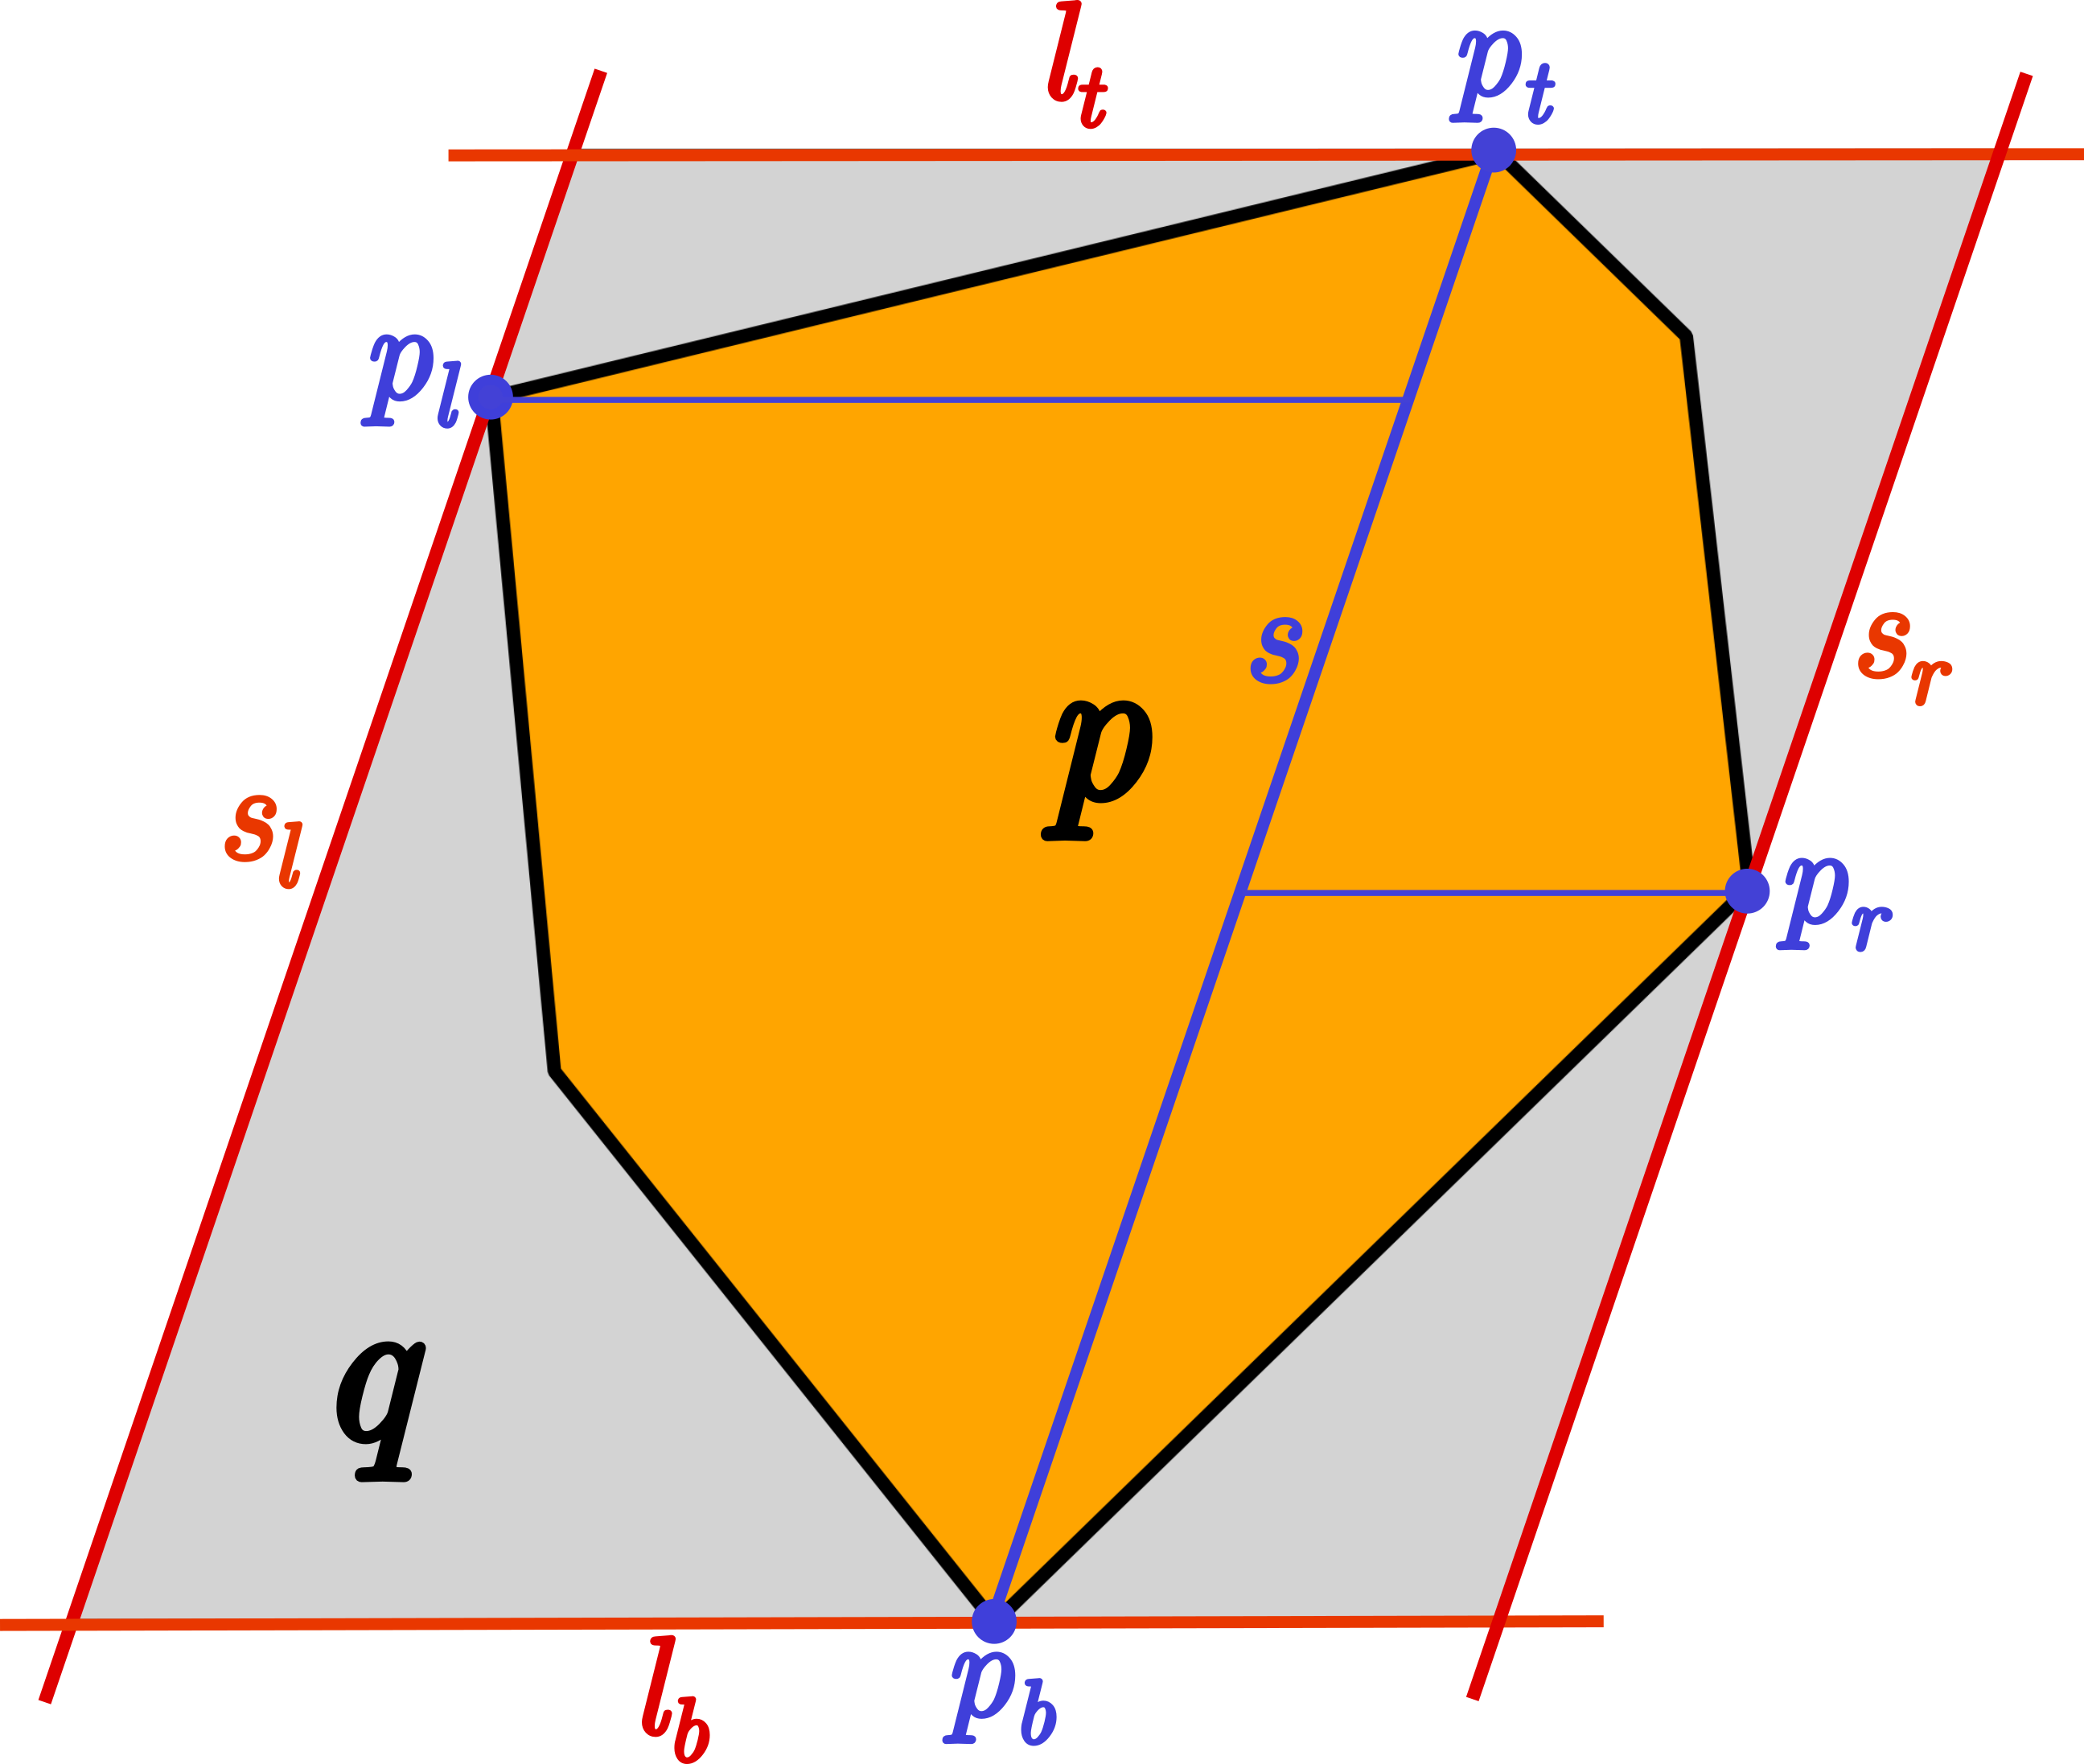
\includegraphics[width=.5\linewidth]{Images/Poly_in_Para_imporved_qual.png}
  \caption{The construction of a bounding parallelogram $q$ from the proof of Lemma \ref{polygon_into_parallelogram} on an example polygon $p$. Note that here, it holds that $\base(q) > \width(p)$.}
  \label{fig_poly_in_para}
\end{figure}

To see that $q$ also satisfies $(iv)$, we consider the triangle with vertices $p_t,p_b$ and $p_l$. We note that it is contained in $p$ due to convexity and contains exactly half the area of the part of $q$ that lies on the left of $s$. Analogously, the triangle with vertices $p_t,p_b$ and $p_r$ has half the area of the part of $q$ that lies on the right of $s$. So $q$ does indeed also satisfy $(iv)$.

However, $q$ does not necessarily satisfy $(ii)$ (see the polygon in Figure \ref{fig_poly_in_para}). If it does, then $q$ satisfies all assumptions of the lemma and we are done.

So we consider now the case when $\base(q) > \width(p)$. Consider the axis-parallel rectangle $r$ bounding $p$. That is, $r$ contains $p$ and each of its sides has non-empty intersection with $p$. Surely $r$ satisfies $(i), (ii)$ and $(iii)$. To see that it also satisfies $(iv)$, note that
%
\begin{align*}
\area(r) &= \width(r) \height(r) \\
&= \width(p) \height(p) \\
& < \base(q) \height(q) \\
& = \area(q) \\
& \leq 2 \area(p).
\end{align*}
%
So whenever $\base(q) > \base(p)$, we showed that $r$ satisfies all requirements $(i)-(iv)$ of the lemma instead. Since $r$ is also an $x$-parallelogram, we conclude.
\end{proof}

With the help of Lemma \ref{polygon_into_parallelogram}, we can now present the main result of this chapter.

\begin{theorem}
\label{polygon_packing_approx}
There is a polynomial time $9.\overline{4}$-approximation algorithm for \textsc{Polygon Area Minimization}. Moreover, there is such algorithm with running time $\mathcal{O}(n^2+N)$, where $n$ is the number of polygons and $N$ the total number of vertices in a given input $I \in \polygons$, assuming that each polygon $p \in I$ is given as a list of its vertices.
\end{theorem}

\begin{proof}
Let $I \in \polygons$. We construct a packing $P$ as the one depicted in Figure \ref{fig_polygon_packing}.

Pack each polygon $p \in I$ into an $x$-parallelogram $q$ as in Lemma \ref{polygon_into_parallelogram}. Call the instance of all so-obtained $x$-parallelograms $I_Q$. The idea of our algorithm is to use FFDH to pack straightened, axis-parallel versions of the $x$-parallelograms $I_Q$ and to then use this packing to obtain one for $I_Q$ and hence also $I$ which is not much bigger.

So, define yet another instance $I_R$ which, for each $q \in I_Q$, contains a rectangle $r=(\base(q),\height(q))$. With FFDH, we now pack $I_R$ into a strip of width $c w_{\max}(I)$, where $c \geq 1$ is to be determined later. Call the so-obtained packing $P_R$. By Theorem \ref{thm:FFDH} it follows
\begin{equation}
\label{area_ffdh_polygon_pack}
\height(P_R)(cw_{\max}(I)) \leq \bigg (1+\frac{1}{m} \bigg)\area(I_R) + c h_{\max}(I_R) w_{\max}(I),  
\end{equation}
where $m = \lfloor c \rfloor$, as $w_{\max}(I_R) = \max_{q \in I_Q} \base(q) \leq w_{\max}(I)$ by Lemma \ref{polygon_into_parallelogram}.

Let $S \subset I_Q$ be the parallelograms corresponding to the rectangles in a certain shelf in the packing $P_R$. We can pack $S$ into a new shelf of width $(c+2)w_{\max}(I)$ by first ordering the parallelograms $S$ by decreasing angle. Indeed, if we, after this ordering, place them all next to each other in the shelf, we note that now all bases of the parallelograms are connected to each other and hence the overlap on either side is at most $\max_{q \in S} \wside(q) \leq w_{\max}(I)$ by Lemma \ref{polygon_into_parallelogram}. Put all such shelves on top of each other and call the so-obtained packing $P_Q$. Note that $P_Q$ has the same height as $P_R$, but $\frac{c+2}{c}$ times its width. Finally, we pack each polygon into its respective parallelogram in the packing $P_Q$. Call this packing $P$. Then
\begin{align*}
\area(P) &\leq \area(P_Q) \\
&\leq \frac{c+2}{c}\height(P_R)(cw_{\max}(I)) \\
& \leq \frac{c+2}{c}\bigg(1+\frac{1}{m}\bigg)\area(I_R) + (c+2) h_{\max}(I_R) w_{\max}(I) \\ 
&= \frac{c+2}{c}\frac{m+1}{m}\area(I_Q) + (c+2) h_{\max}(I_Q) w_{\max}(I) \\ 
& \leq 2 \frac{c+2}{c} \frac{m+1}{m} \area(I) + (c+2) h_{\max}(I) w_{\max}(I) \\
& \leq \bigg ( 2\frac{c+2}{c}\frac{m+1}{m}+(c+2) \bigg) \opt(I).
\end{align*}
One can check that the minimum is attained at $c=3$, in which case we get a $9.\overline{4}$-approximation.

\begin{figure}[h]
\centering
  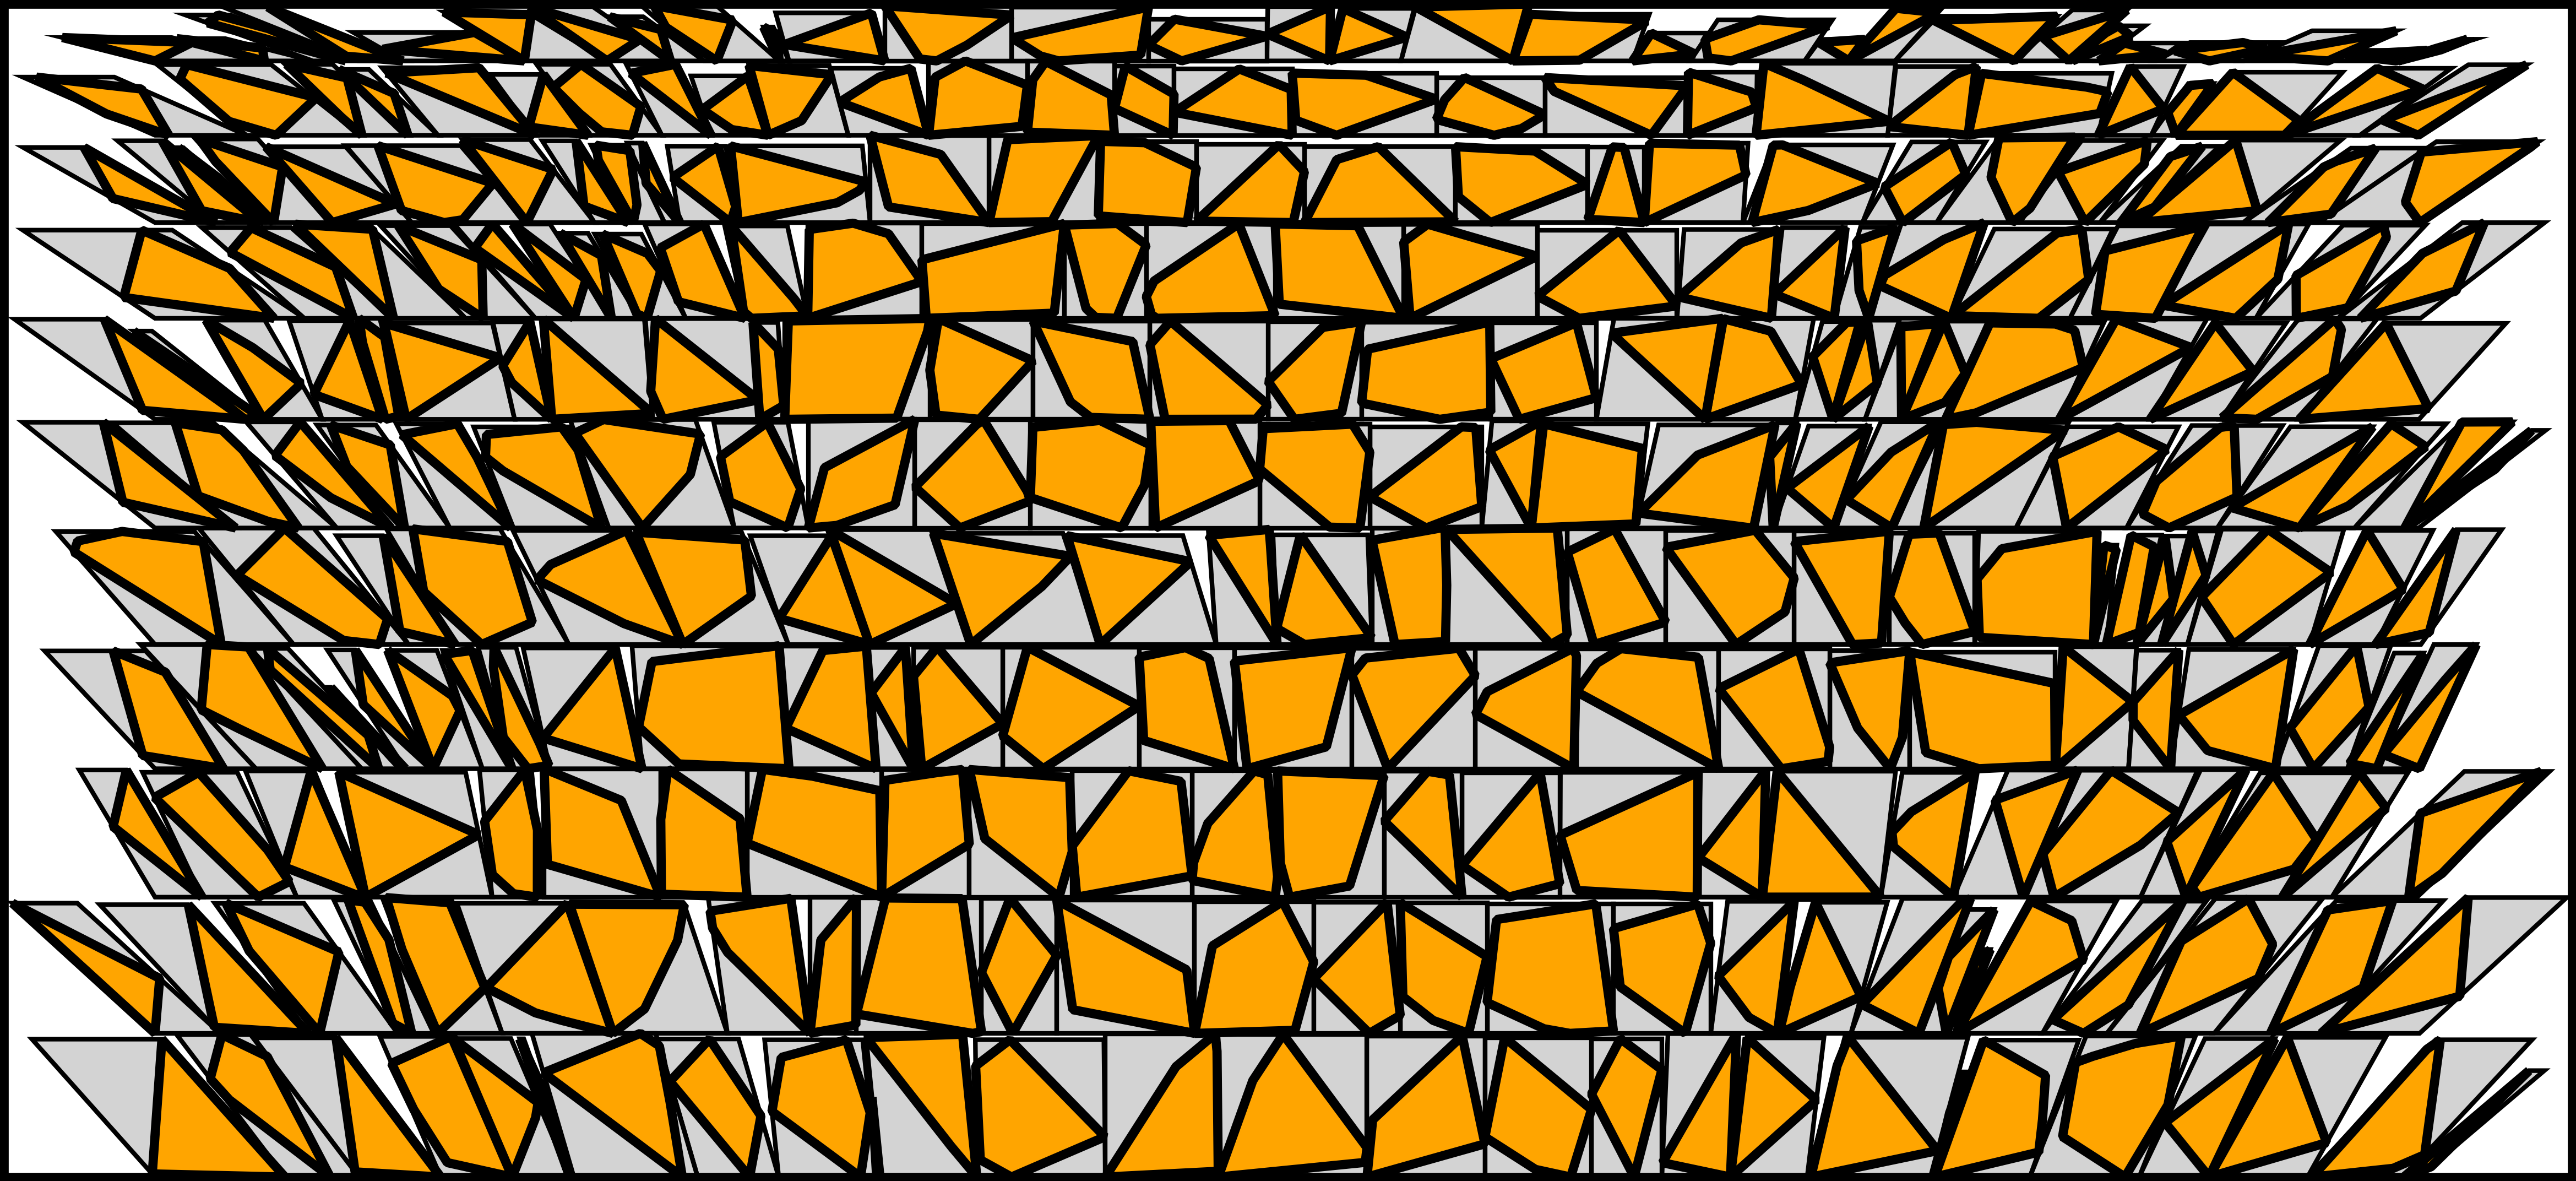
\includegraphics[width=.7\linewidth]{Images/bigger_instance.png}
  %\includegraphics[width=.7\linewidth]{lipics-authors-v2021/Images/2023-03-12_example_poly_packing2.png}
  \caption{A packing computed with the algorithm from the proof of Theorem \ref{polygon_packing_approx}, here with parameter $c=15$. For each polygon, also its computed bounding $x$-parallelogram is drawn.}
  \label{fig_polygon_packing}
\end{figure}

We now note that the claimed running times of the above algorithm follows by observing that: Constructing $I_Q$ from $I$ can be done in $\mathcal{O}(N)$ time, constructing $I_R$ from $I_Q$ can be done in $\mathcal{O}(n)$ time, constructing $P_R$ can be done in $\mathcal{O}(n^2)$ time, constructing $P_Q$ from $P_R$ can be done by sorting in $\mathcal{O}(n \log(n))$ time, and finally, constructing $P$ from $P_Q$ can be done in $\mathcal{O}(N)$ time.
\end{proof}

The algorithm of Alt et al. runs in time $\mathcal{O}(N \log(N))$ and thus for certain instances faster than our algorithm. If, in our algorithm, the use of FFDH for packing $I_R$ is replaced by NFDH, one can show using Theorem \ref{nfdh} that for an optimal choice of $c=2 \sqrt{2}$, the algorithm has an approximation guarantee of 11.66 while having a running time of $\mathcal{O}(n \log(n) + N)$, thus obtaining an algorithm that runs faster than the algorithm of Alt et al., while still having a greatly improved approximation ratio.

% We do now show the claimed running time of the above algorithm. For this, we prove the following statements.
% \begin{enumerate}
%     \item Constructing $I_Q$ from $I$ can be done in $\mathcal{O}(N)$ time.
%     \item Constructing $I_R$ from $I_Q$ can be done in $\mathcal{O}(n)$ time.
%     \item Constructing $P_R$ can be done in $\mathcal{O}(n^2)$ time.
%     \item Constructing $P_Q$ from $P_R$ can be done in $\mathcal{O}(n \log(n))$ time.
%     \item Constructing $P$ from $P_Q$ can be done in $\mathcal{O}(N)$ time.
% \end{enumerate}
% \textbf{(i)}. Let $p \in I$ and set $N_p := \lvert \vertices(p) \rvert$. To construct a spine $s$, we have to find vertices $p_t$ and $p_b$ with maximum and minimum $y$-coordinate. This can be done in $\mathcal{O}(N_p)$ time. Let $\overline{s}$ be normal to $s$ with $\langle \overline{s},e_1 \rangle > 0$, where $\langle \cdot, \cdot \rangle$ is the standard dot product in $\R^2$. Points $p_l \in \argmax_{v \in \vertices(p)} \langle \overline{s},v \rangle$ and $p_r \in \argmin_{v \in \vertices(p)} \langle \overline{s},v \rangle$ can be found in time $\mathcal{O}(N_p)$ as well. From here, the bounding parallelogram $q$ can now be constructed in constant time. To compute $\width(p)$, we compute in time $\mathcal{O}(N_p)$ the left- and rightmost vertices of $p$. Having already computed the points in $p$ with maximum and minimum $x$- and $y$-coordinates, the bounding rectangle $r$ can be constructed in constant time, if $\width(p) > \base(q)$. Hence, for all polygons $I$, we see that time $\sum_{p \in I} \mathcal{O}(N_p) = \mathcal{O}(N)$ is sufficient for this step.

% \textbf{(ii)}. Height and base of a parallelogram $q \in I_Q$ can be computed in time $\mathcal{O}(1)$ from $p_t, p_b, p_l$ and $p_r$ and hence for all polygons, this step can be done in time $\mathcal{O}(n)$. For each polygon $p$, safe the position of one of its vertices inside its corresponding parallelogram $q$ for step $(v)$.

% \textbf{(iii)}. Computing $w_{\max}(I)$ needs time $\mathcal{O}(n)$. The rectangles in $I_R$ need to be sorted by height, which needs time $\mathcal{O}(n\log(n))$. The time for packing the rectangles after sorting by height can be bounded by $\mathcal{O}(n^2)$. Indeed, when FFDH considers a rectangle $r \in I_R$, it tests from the bottom shelf upwards if $r$ fits. The number of opened shelves at the time $r$ is considered is upper bounded by $n$.

% \textbf{(iv)}. Computing the angle of the slope of a parallelogram needs constant time. The sorting of the parallelograms by slope in each shelf can be done in time $\mathcal{O}(n\log(n))$.

% \textbf{(v)}. Packing the polygons into their respective parallelogram in the packing $P_Q$ needs $\mathcal{O}(N)$ time, assuming that we stored the location of at least one vertex of any polygon in its respective parallelogram in step $(ii)$. From the position of one vertex of a polygon in the packing $P$, we can easily compute the position of all others.


%%%%%%%%%%%%%%%%%%%%%%%%%%%%%%%%%%%%%%%%%%%%%%%%%%%%%%%%%%%%%%%%%%%%%%
%%%%%%%%%%%%%%%%%%%  deleted for conference version %%%%%%%%%%%%%%%%%%
%%%%%%%%%%%%%%%%%%%%%%%%%%%%%%%%%%%%%%%%%%%%%%%%%%%%%%%%%%%%%%%%%%%%%%
% \begin{remark}
% The algorithm from Theorem \ref{polygon_packing_approx} can be made faster at the cost of potentially having a bit of a worse approximation ratio. Indeed, if we pack $I_0$ with NFDH instad of FFDH, step $(iii)$ in the time complexity analysis above only needs time $\mathcal{O}(n \log (n))$ and hence the complete algorithm's running time reduces to $\mathcal{O}(N + n \log(n))$. In this case, one can check that one gets an approximation ratio of $6+4 \sqrt{2} \approx 11.66$ for $c=2\sqrt{2}$ (using Theorem \ref{nfdh}, not leveraging the bounded width of the rectangles with respect to the width of the strip).

% On the other hand, the algorithm can also be improved so as to give a better approximation of the optimal solution for many instances $I \in \polygons$. Indeed, when using FFDH, for a given shelf $S$, one can already keep track of the maximum wsides among all parallelogram that are tilted to the left and also of those tilted to the right, from which the rectangles in $S$ are constructed. Then, one can add rectangles to the shelf as long as the total length of the bases plus those two numbers are smaller than $(c+2)w_{max}(I)$. \newline
% Even going a step further, instead of packing rectangles with FFDH altogether, one could also directly pack the polygons with a FFDH-type heuristic for a predetermined strip-width $W \geq w_{\max}(I)$. Precisely, one could consider the following shelf-packing algorithm for $I= \{p_1, \dots, p_n\}$. Place $p_1$ into the lowest shelf. Let $l \in [n]$ and assume that $p_i$ was placed for all $i \in [l-1]$. Then, when placing $p_l$, check if it fits into any already opened shelf (starting from the lowest) in the following way. For a given shelf, find the polygon $p$, so that the angle of $p_l$ is smaller than the angle of $p$ but all polygons coming after $p$ (if any) have smaller angle than $p_l$. After finding this place, place the polygon to the right of $p$ as closely as possibly, while keeping $p_l$ and $p$ touching the floor of the shelf (and thus keeping the shelf to be a proper shelf of a shelf-packing according to Definition \ref{def_poly_shelf_packing}), and place the polygons that were on the right of $p$ to the right of $p_l$ instead, again in the closest way possible. If the width of this new packing of the shelf still fits into the predetermined shelf-width $W$, we can place $p_l$ like this (and hence also change the placements of all polygons that were on the right of $p$). If it is not possible to place it in any shelf in such a way, open a new shelf above the last opened one. \newline
% Both of these methods can be shown to not have a worse approximation guarantee than our algorithm, but we do not know if they can achieve a better one.
% \end{remark}
%%%%%%%%%%%%%%%%%%%%%%%%%%%%%%%%%%%%%%%%%%%%%%%%%%%%%%%%%%%%%%%%%%%%%%%%%%%%

\subsection{An Efficient $7$-Approximation for \textsc{Polygon Area Minimization} when all Polygons are $x$-Parallelograms}
\label{section_x_parallelogram_areamin}

In the algorithm presented in the previous subsection, we first pack general polygons into $x$-parallelograms and afterwards pack these $x$-parallelograms. One would expect that if one wants to pack $x$-parallelograms from the start, one should be able to obtain a better approximation factor. Showing that this is indeed the case is the content of this brief section.

\begin{theorem}
There is a polynomial time $7$-approximation algorithm for \textsc{Polygon Area Minimization}, when all input polygons are $x$-parallelograms.
\end{theorem}

The proof follows along the lines of the proof of Theorem \ref{polygon_packing_approx}.

\begin{proof}
Let $I \in \polygons$ be so that every $p \in I$ is an $x$-parallelogram. As in the proof of Theorem \ref{polygon_packing_approx}, we define the set $I_R \in \rectangles$ that for every $p \in I$ contains some $r \in I_R$ with $\width(r) = \base(p)$ and $\height(r) = \height(p)$. Again, we pack $I_R$ with FFDH into a strip of width $cw_{\max}(I)$ and call the so-obtained packing $P_R$.

After ordering them by angle, we can pack the parallelograms $S \subset I$ corresponding to the rectangles in some shelf in $P_R$ into a new shelf of width $(c+2)w_{\max}(I)$, because of course $\wside(p) \leq w_{\max}(I)$. Therefore, calling the so-obtained packing $P$,
\begin{align*}
    \area(P) &\leq \frac{c+2}{c}\area(P_R) \\
    & \leq \frac{c+2}{c}\frac{m+1}{m}\area(I) + (c+2)h_{\max}(I)w_{\max}(I) \\
    & \leq \bigg( \frac{c+2}{c}\frac{m+1}{m} + (c+2) \bigg) \opt(I),
\end{align*}
which, for $c=2$, is minimized and equal to $7$.
\end{proof}

\section{An Efficient $(3.75+\epsilon)$-Approximation for \textsc{Polygon Perimeter Minimization} and $(3.56+\epsilon)$-Approximation for \textsc{Polygon Minimum Square}}
\label{section_polygon_perimeter_min}

In this section, we show how to leverage the algorithm from Theorem \ref{polygon_packing_approx} to obtain an approximation-algorithm for \textsc{Polygon Perimeter Minimization}. We improve on the polynomial time $7.3$-approximation algorithm obtained by Aamand et al. \cite{aamand_23} and present an efficient $(3.75 + \epsilon)$-approximation. Moreover, we show how to leverage that result to obtain an $(3.56+\epsilon)$-approximation-algorithm for \textsc{Polygon Minimum Square}.

\subsection{An Efficient $(3.75+\epsilon)$-Approximation for \textsc{Polygon Perimeter Minimization}}

\begin{theorem}
\label{polygon_perimeter_min}
For every $\epsilon>0$, there is an efficient $(3.75+\epsilon)$-approximation algorithm for \textsc{Polygon Perimeter Minimization}.
\end{theorem}

\begin{proof}
Let $I \in \polygons$. Note that for the perimeter objective, it surely holds that
\begin{equation}
\label{opt_perimeter_vs_wmax_hmax}
\opt(I) \geq 2(w_{\max}(I) + h_{\max} (I)).
\end{equation}
Furthermore, since a bounding box of $I$ has area at least $\area(I)$ and the minimum perimeter rectangle having area $\area(I)$ is a square, it also is true that
\[
\opt(I) \geq 4 \sqrt{\area(I)}.
\]
It follows from Inequality \ref{opt_perimeter_vs_wmax_hmax} that
\[
\min \{h_{\max}(I),w_{\max}(I)\} \leq \frac{1}{4}\opt(I)
\]
and without loss of generality, we assume that $w_{\max}(I) \leq \frac{1}{4}\opt(I)$. Otherwise we are making the following argument by packing into vertical shelves instead.

Let $P$ be the packing obtained from the algorithm in Theorem \ref{polygon_packing_approx}, leaving $c$ as a free parameter. Then $P$ satisfies
\[
\width(P) \leq (c+2)w_{\max}(I)
\]
and by dividing the inequality (\ref{area_ffdh_polygon_pack}) by the width of the strip used for the rectangle packing obtained by FFDH, $cw_{\max}(I)$, we see that
\[
\height(P) \leq 2 \frac{m+1}{m} \frac{\area(I)}{cw_{\max}(I)} + h_{\max}(I) \leq \frac{1}{8} \frac{m+1}{m} \frac{\opt(I)^2}{cw_{\max}(I)} + h_{\max}(I).
\]
We restrict the domain of $c$ so that $c \geq \frac{\opt(I)}{4w_{\max}(I)} \geq 1$ and write $c = l \frac{\opt(I)}{4w_{\max}(I)}$ for some $l \geq 1$. Then
\[
\width(P) \leq \frac{l}{4} \opt(I) + 2w_{\max}(I), \quad \height(P) \leq \frac{1}{2l}\frac{m+1}{m} \opt(I) + h_{\max}(I).
\]
The perimeter of $P$ is hence bounded by
\begin{align*}
2(\width(P) + \height(P)) &\leq 2 \bigg( \bigg(\frac{l}{4} + \frac{m+1}{2lm} \bigg) \opt(I) + 2w_{\max}(I) + h_{\max}(I) \bigg) \\
& \leq 2 \bigg ( \frac{1}{4} \bigg(l + \frac{2(m+1)}{lm} \bigg) + 1 \bigg) \opt(I) \\
& = \frac{1}{2} \bigg( l+\frac{2(m+1)}{lm} + 4 \bigg) \opt(I),
\end{align*}
which is minimized and equal to $3.75 \opt(I)$ when $l$ is equal to $\overline{l}:=2$, where we used that $m = \lfloor c \rfloor \geq \lfloor l \rfloor$.

Now since the value of $\opt(I)$ is not known beforehand and since $\overline{l}$ depends on it, we need to guess an optimal value for $l$. This can be done as follows. Compute the packing from the algorithm in Theorem \ref{polygon_packing_approx} for $c=1,(1+\epsilon), \dots, (1+\epsilon)^K$, where $K=\frac{\log(n)}{\log(1+\epsilon)}$ and denote the packing obtained for $c=(1+\epsilon)^k$ by $P_k$ for all $k \in \{0,1, \dots, n\}$. Over all those packings, choose the one that has minimum perimeter. Say this perimeter is $z > 0$. Let $k \in \{1, \dots, K\}$ be so that
\[
(1+\epsilon)^{k-1} \leq \overline{c} \leq (1+\epsilon)^{k},
\]
where $\overline{c} := \overline{l} \frac{\opt(I)}{4w_{\max}(I)}$. Then, for $l_k := (1+\epsilon)^k \frac{4w_{\max}(I)}{\opt(I)}$, it holds that
\[
l_k = (1+\epsilon)^k \frac{4w_{\max}(I)}{\opt(I)} \leq (1+\epsilon) \overline{c}\frac{4w_{\max}(I)}{\opt(I)} = (1+\epsilon)\overline{l}.
\]
In particular, as of course also $\overline{l} \leq l_k$, it holds that
\begin{align*}
z & \leq 2(\width(P_k) + \height(P_k)) \\
&\leq \frac{1}{2} \bigg( l_k+\frac{2(m+1)}{l_km} + 4 \bigg) \opt(I) \\
&\leq (1+\epsilon) \frac{1}{2} \bigg( \overline{l}+\frac{2(m+1)}{\overline{l}m} + 4 \bigg) \opt(I) \\
&\leq (1+\epsilon)3.75 \opt(I),
\end{align*}
which shows the statement.
\end{proof}


\subsection{An Efficient $(3.56+\epsilon)$-Approximation for \textsc{Polygon Minimum Square}}
\label{section_polygon_min_square}

In this section, we show how to leverage the algorithm from Theorem \ref{polygon_packing_approx} to obtain an approximation-algorithm for \textsc{Polygon Minimum Square}.

\begin{theorem}
For every $\epsilon>0$, there is an efficient $(3.56+\epsilon)$-approximation algorithm for \textsc{Polygon Minimum Square}.
\end{theorem}

The proof is similar to the proof of Theorem \ref{polygon_perimeter_min}.

\begin{proof}
Let $I \in \polygons$. Note that
\[
\opt(I) \geq \max\{w_{\max}(I),h_{\max}(I)\}
\]
and also
\[
\opt(I) \geq \sqrt{\area(I)}.
\]
Analogously to the proof of Theorem \ref{polygon_perimeter_min}, but substituting $c=l\frac{\opt(I)}{w_{\max}(I)}$ for some $l \geq 1$ instead, we can construct a packing $P$ with
\[
\width(P) \leq l \opt(I) + 2w_{\max}(I), \quad \height(P) \leq \frac{2}{l}\frac{m+1}{m}\opt(I) + h_{\max}(I).
\]
Then
\[
\max\{\width(P),\height(P)\} \leq \max \bigg\{l+2,\frac{2(m+1)}{lm}+1 \bigg\} \opt(I).
\]
The minimum is attained for $l=\overline{l}:=\frac{1}{2}(\sqrt{17}-1)$ in which case $m=1$ and the approximation factor is equal to to $\frac{1}{2}(\sqrt{17}+3) \approx 3.56$. As in the proof of Theorem \ref{polygon_perimeter_min}, we can guess the value of $\overline{l}$ to obtain a $(3.56+\epsilon)$-approximation algorithm.
\end{proof}

% \section{Other Polygon Packing Problems}
% \label{chapter_further_polygon}

% In this chapter, we consider \textsc{Polygon Strip Packing} and \textsc{Polygon Bin Packing} and give new approximability results for both.

\section{An Efficient $21.89$-Approximation for \textsc{Polygon Strip Packing}}
\label{section_polygon_strip}

In this section, we show how to obtain a polynomial time $21.\overline{8}$-approximation for \textsc{Polygon Strip Packing}, improving on the previous best known approximation factor for efficient algorithms of $51$ by Aamand et al. \cite{aamand_23}.
%
% Contrary to \textsc{Strip Packing} for rectangles, there does not exist a shelf-packing algorithm for \textsc{Polygon Strip Packing} with constant approximation ratio, as the following example shows.
%
% \begin{example}
% Consider an instance consisting of $n$ $x$-parallelograms, each of which with width $1$, height $1$ and base of length $\epsilon$. The optimal shelf-packing solution for a strip-width of $1$ has height at least $n$. The optimal strip packing solution, however, is obtained from the optimal shelf packing solution by pushing down each parallelogram as far as possible. Note that the slope of the left and right sides of any one of the $x$-parallelogram is $\frac{1}{1-\epsilon}$. Thus, if one of them has its base at height $h$, the one above it in the optimal packing has its base at height $h + \frac{\epsilon}{1-\epsilon}$. Hence the optimal packing has height $1 + \frac{n \epsilon}{1-\epsilon}$. Letting $\epsilon \searrow 0$ shows that each shelf-packing has height at least $n \opt$.
% \end{example}
%
% The example illustrates that shelf-packing is not a valid approach for \textsc{Polygon Strip Packing} in order to obtain a constant factor approximation. If the widths of the input polygons are bounded by a fraction of the width of the strip, this is different. Indeed, if, for example, the widths of the polygons are bounded by $\frac{1}{3}$, we can use the algorithm from Theorem \ref{polygon_packing_approx} with $c=1$. Slightly altering the algorithm, packing only left-tilted or only right-tilted polygons into a given shelf, we can also use the algorithm if the widths of the polygons are bounded by $\frac{1}{2}$. We will discuss this idea more in the context of \textsc{Polygon Bin Packing} in the next section.
%
% In the following, we discuss another approach on how to leverage our algorithm, which works for polygons of arbitrary widths. 
The idea is to construct vertical shelves with the algorithm from Theorem \ref{polygon_packing_approx} and then to stack such vertical shelves horizontally into the strip. This idea comes from \cite{aamand_23}. We slightly improve their procedure using the following observation.

\begin{lemma}
\label{split_shelf}
Let $\overline{I} \in \polygons$ and let $\overline{P} \subset [0,(c+2)w_{\max}(\overline{I})] \times [0, \infty)$ be a shelf-packing obtained by the algorithm from Theorem \ref{polygon_packing_approx} for some $c \geq 1$. Let $I \subset \overline{I}$ be the polygons in one of the shelves of $\overline{P}$ and define the packing $P:=\{\overline{P}(p)\}_{p \in I}$. Then there is a shelf-packing $P'$ of $I$ into two shelves with $\width(P') \leq \frac{1}{2}(c+3)w_{\max}(\overline{I})$ and $\height(P') \leq 2\height(P)$.
\end{lemma}

\begin{proof}
The idea is to simply split the shelf in half in its middle as follows. Let $x_{\text{mid}} := \frac{(c+2)w_{\max}(\overline{I})}{2}$ and partition $I$ into the two sets
\[
I_L:=\bigg \{p \in I \, | \, \width \big(P(p) \cap (\R_{\geq x_{\text{mid}}} \times \R) \big) \leq \frac{\width(p)}{2} \bigg \}
\]
and $I_R = I \backslash I_L$. Note that
\[
I_R \subset \bigg \{p \in I \, | \, \width \big(P(p) \cap (\R_{\leq x_{\text{mid}}} \times \R) \big) < \frac{\width(p)}{2}\bigg\}.
\]
We can now pack $I_L$ and $I_R$ into separate shelves while respecting the ordering of the polygons in $P$. We denote the packing where both of those shelves are stacked on each other by $P'$. Both shelves have width at most
\[
x_{\text{mid}} + \frac{w_{\max}(I)}{2} \leq x_{\text{mid}} + \frac{w_{\max}(\overline{I})}{2} = \frac{1}{2}(c+3)w_{\max}(\overline{I}).
\]
and hence $P'$ does as well.
\end{proof}

Making use of the lemma, we can show the following result.

\begin{theorem}
There is a polynomial time $21.\overline{8}$-approximation algorithm for \textsc{Polygon Strip Packing}.
\end{theorem}

\begin{proof}
Let $I \in \polygons$. We apply the algorithm from Theorem \ref{polygon_packing_approx}, for some $c$ which we will fix later, to construct vertical shelves. More precisely, we rotate each item by an angle of $\pi/2$, apply the algorithm to the rotated instance, and then rotate the whole packing back by $\pi/2$. Let $P$ be the so obtained packing and let $S_1, \dots, S_k$ be the vertical shelves of this packing.

We now stack $S_1, \dots, S_k$ horizontally into the (vertical) strip. That is, we pack the $\{S_i\}_{i \in [k]}$ into horizontal shelves $T_1, \dots, T_l$ themselves. Note that since each shelf $S_i$, where $i \in [k]$, has the same height, the problem reduces to $(1D)$-\textsc{Bin Packing}. In particular, stacking the $\{S_i\}_{i \in [k]}$ greedily, each except for possibly the last horizontal shelf is covered by at least half by the $S_i$. If the last shelf $T_l$ is covered by half, we need at most $l \leq \frac{2\area(P)}{(c+2)h_{\max}(I)}$ horizontal shelves to pack $S_1, \dots, S_k$. Otherwise, we need at most $l \leq \frac{2\area(P)}{(c+2)h_{\max}(I)}+1$ shelves. However, in this case we can reduce the height of $T_l$, which is filled less than half by the $\{S_i\}_{i \in [k]}$, to $\frac{1}{2}(c+3)h_{\max}(I)$ by using Lemma \ref{split_shelf} on every shelf $S$ in $T_l$.

In particular, for such packing $P'$ it holds that
\begin{align*}
\height(P') &\leq \bigg( \frac{2\area(P)}{(c+2)h_{\max}(I)} \bigg) (c+2)h_{\max}(I) + \frac{1}{2}(c+3) h_{\max}(I) \\
&= 2\area(P) + \frac{1}{2}(c+3)h_{\max}(I) \\
&\leq \bigg ( 4\frac{c+2}{c}\frac{m+1}{m}+\frac{5}{2}c + \frac{11}{2} \bigg) \opt(I) \\
& = 21.\overline{8} \opt(I),
\end{align*}
which is attained for $c = 3$.
\end{proof}

% \begin{remark}
% For practical application, the arising ($1D$)-\textsc{Bin Packing} problem can for example be solved with \textsc{First Fit Decreasing} or another \textsc{Bin Packing}-algorithm instead of the greedy \textsc{Next Fit Decreasing} approach used in the proof in order to obtain better results. We do, however, not know how this could lead to a better worst case approximation guarantee.
% \end{remark}

\section{Efficient Approximation Algorithms for \textsc{Polygon Bin Packing} for Polygons of Width Upper Bounded by $1/M$}
\label{section_polygon_1/M}

In this section, we present polynomial time approximation algorithms for \textsc{Polygon Bin Packing} for the case when polygons have their width bounded by a fraction of the form $\frac{1}{M}$ and also improved approximations if their height is bounded as well.

To the best of our knowledge, the only presently published polynomial time approximation algorithm for \textsc{Polygon Bin Packing} is an $11$-approximation in the case when the diameter of the input polygons is bounded by $\frac{1}{10}$, see \cite{aamand_23}. For this case, we obtain an efficient $5.09$-approximation.

We prove the following theorem.

\begin{theorem}
\label{polygon_bin_packing_1/M}
Let $I \in \polygons$ and assume that there is some $M \in \N_{\geq 2}$ with $w_{\max}(I) \leq \frac{1}{M}$. Then one can pack $I$ into
\[
\begin{cases}
32 \opt(I) + 5 & \text{if $M=2$} \\
\frac{4M(M-1)}{(M-2)^2}\opt(I) + 3 & \text{if $M \geq 3$}
\end{cases}
\]
bins efficiently. If additionally $h_{\max}(I) \leq \frac{1}{M}$, then we can even efficiently pack $I$ into
\[
\begin{cases}
24 \opt(I) + 3 & \text{if $M=2$} \\
\frac{2(M+1)(M-1)}{(M-2)^2}\opt(I)+2 & \text{if $M \geq 3$}
\end{cases}
\]
bins.
\end{theorem}

In particular, for inputs where both width and height of all polygons are upper bounded by $\frac{1}{10}$, we get a $5.09$-approximation.

\begin{proof}
Assume first that $M \geq 3$. We use the algorithm from Theorem \ref{polygon_packing_approx} for $c=\frac{1}{w_{\max}(I)}-2 \geq M-2$ to obtain a packing $P$ with shelves $S_1, \dots, S_k$. The packing $P$ satisfies
\[
\width(P) \leq (c+2)w_{\max}(I) = 1,
\]
and hence a shelf $S_i$, $i \in [k]$, fits into a unit bin. Note that $m = \lfloor c \rfloor \geq M-2$, since $M-2$ is an integer. Since $cw_{\max}(I) = 1-2w_{\max}(I) \geq \frac{M-2}{M}$, it holds that
\[
\height(P) \leq 2\bigg(1+\frac{1}{m}\bigg)\frac{\area(I)}{cw_{\max}(I)} + h_{\max}(I) \leq 2\bigg(1+\frac{1}{M-2}\bigg)\frac{\area(I)}{(M-2)/M} + h_{\max}(I).
\]
We can now use NF to distribute the shelves into unit bins. Since $h_{max} = 1$, this uses at most $2\height(P)+1$ bins, see Section \ref{section:shelf_packing}. But
\[
2 \height(P) + 1 \leq 4\bigg(1+\frac{1}{M-2}\bigg) \frac{\area(I)}{(M-2)/M} + 2h_{\max}(I) + 1 \leq \frac{4M(M-1)}{(M-2)^2}\opt(I) + 3.
\]

If $h_{\max}(I) \leq \frac{1}{M}$ as well, we can use FF instead of NF to distribute the shelves into bins, which needs at most $(1+\frac{1}{M})\height(P)+1$ bins, see again Section \ref{section:shelf_packing}. This way, the number of needed bins is bounded by
\[
\bigg(1+\frac{1}{M}\bigg) \height(P) + 1 \leq \frac{2(M+1)(M-1)}{(M-2)^2}\opt(I)+2,
\]
as claimed.

Now we consider the case when $M=2$. Partition $I$ into two sets $I_L$ and $I_R$, where a polygon $p \in I$ belongs to $I_L$ if its chosen $x$-parallelogram in the proof of Theorem \ref{polygon_packing_approx} is tilted to the left and to $I_R$ if it is tilted to the right. We now proceed with the algorithm in the proof of Theorem \ref{polygon_packing_approx} for $c=\frac{1}{w_{max}(I)} - 1 \geq 1$, but for $I_L$ and $I_R$ separately. Call the obtained packings $P_L$ and $P_R$, respectively. Note that since all are tilted to one side only,
\[
\width(P_L), \, \width(P_R) \leq (c+1)w_{\max}(I) = 1
\]
and, using $m=\lvert c \rvert \geq 1$ and $cw_{\max}(I) = 1-w_{\max}(I) \geq \frac{1}{2}$,
\[
\height(P_L) \leq 2\bigg(1+\frac{1}{m}\bigg)\frac{\area(I_L)}{cw_{\max}(I_L)} + h_{\max}(I_L) \leq 8\area(I_L) + h_{\max}(I),
\]
as well as analogously $\height(P_R) \leq 8 \area(I_R) + h_{\max}(I)$.

Hence, for the packing $P$, where $P_R$ is stacked on top of $P_L$, it holds that
\[
\width(P) \leq 1 \quad \text{and} \quad \height(P) \leq 16 \area(I) + 2 h_{\max}(I).
\]
From here, with the same arguments as for $M \geq 3$, we obtain the desired bounds.
\end{proof}

\section{Efficient Approximations for \textsc{Polygon Bin Packing} for Polygons with bounded Width or Height and for Instances, where each Polygon has a Spine from a Set of Constant Size}
\label{section_polygon_bin_pack}


In this last section, we give further results on \textsc{Polygon Bin Packing}, attempting to further close the gap towards the question of an efficient $\mathcal{O}(1)$-approximation.

\subsection{An Efficient $\mathcal{O}(\frac{1}{\delta})$-Approximation for \textsc{Polygon Bin Packing} for Polygons with Width or Height at Most $1-\delta$}
\label{section_polygon_1-delta}

We now also consider wider polygons than in Section~\ref{section_polygon_1/M} and prove the following result.

\begin{theorem}
\label{polygon_bin_packing_1_minus_delta}
There is an efficient $\mathcal{O}(\frac{1}{\delta})$-approximation algorithm for \textsc{Polygon Bin Packing} for instances $I \in \polygons$, where each $p \in I$ satisfies $\width(p) \leq 1-\delta$ or $\height(p) \leq 1- \delta$.
\end{theorem}

The result leaves the question whether \textsc{Polygon Bin Packing} admits a $\mathcal{O}(1)$-approximation algorithm open. To obtain an affirmative proof, one is left to provide, for any fixed $\delta>0$, an $\mathcal{O}(1)$-approximation algorithm for polygons $p$ that satisfy both $\width(p) \geq 1-\delta$ and $\height(p) \geq 1-\delta$. We will use and see in the proof, that additionally, one can easily pack polygons with area bigger than some fixed threshold $\eta > 0$. Thus, only polygons that are wide, high and have small area (see Figure \ref{image_problematic_polygon}) are problematic for our described methods. We will present some ideas to deal with such polygons in the coming, last section.

\begin{figure}[h]
\centering
  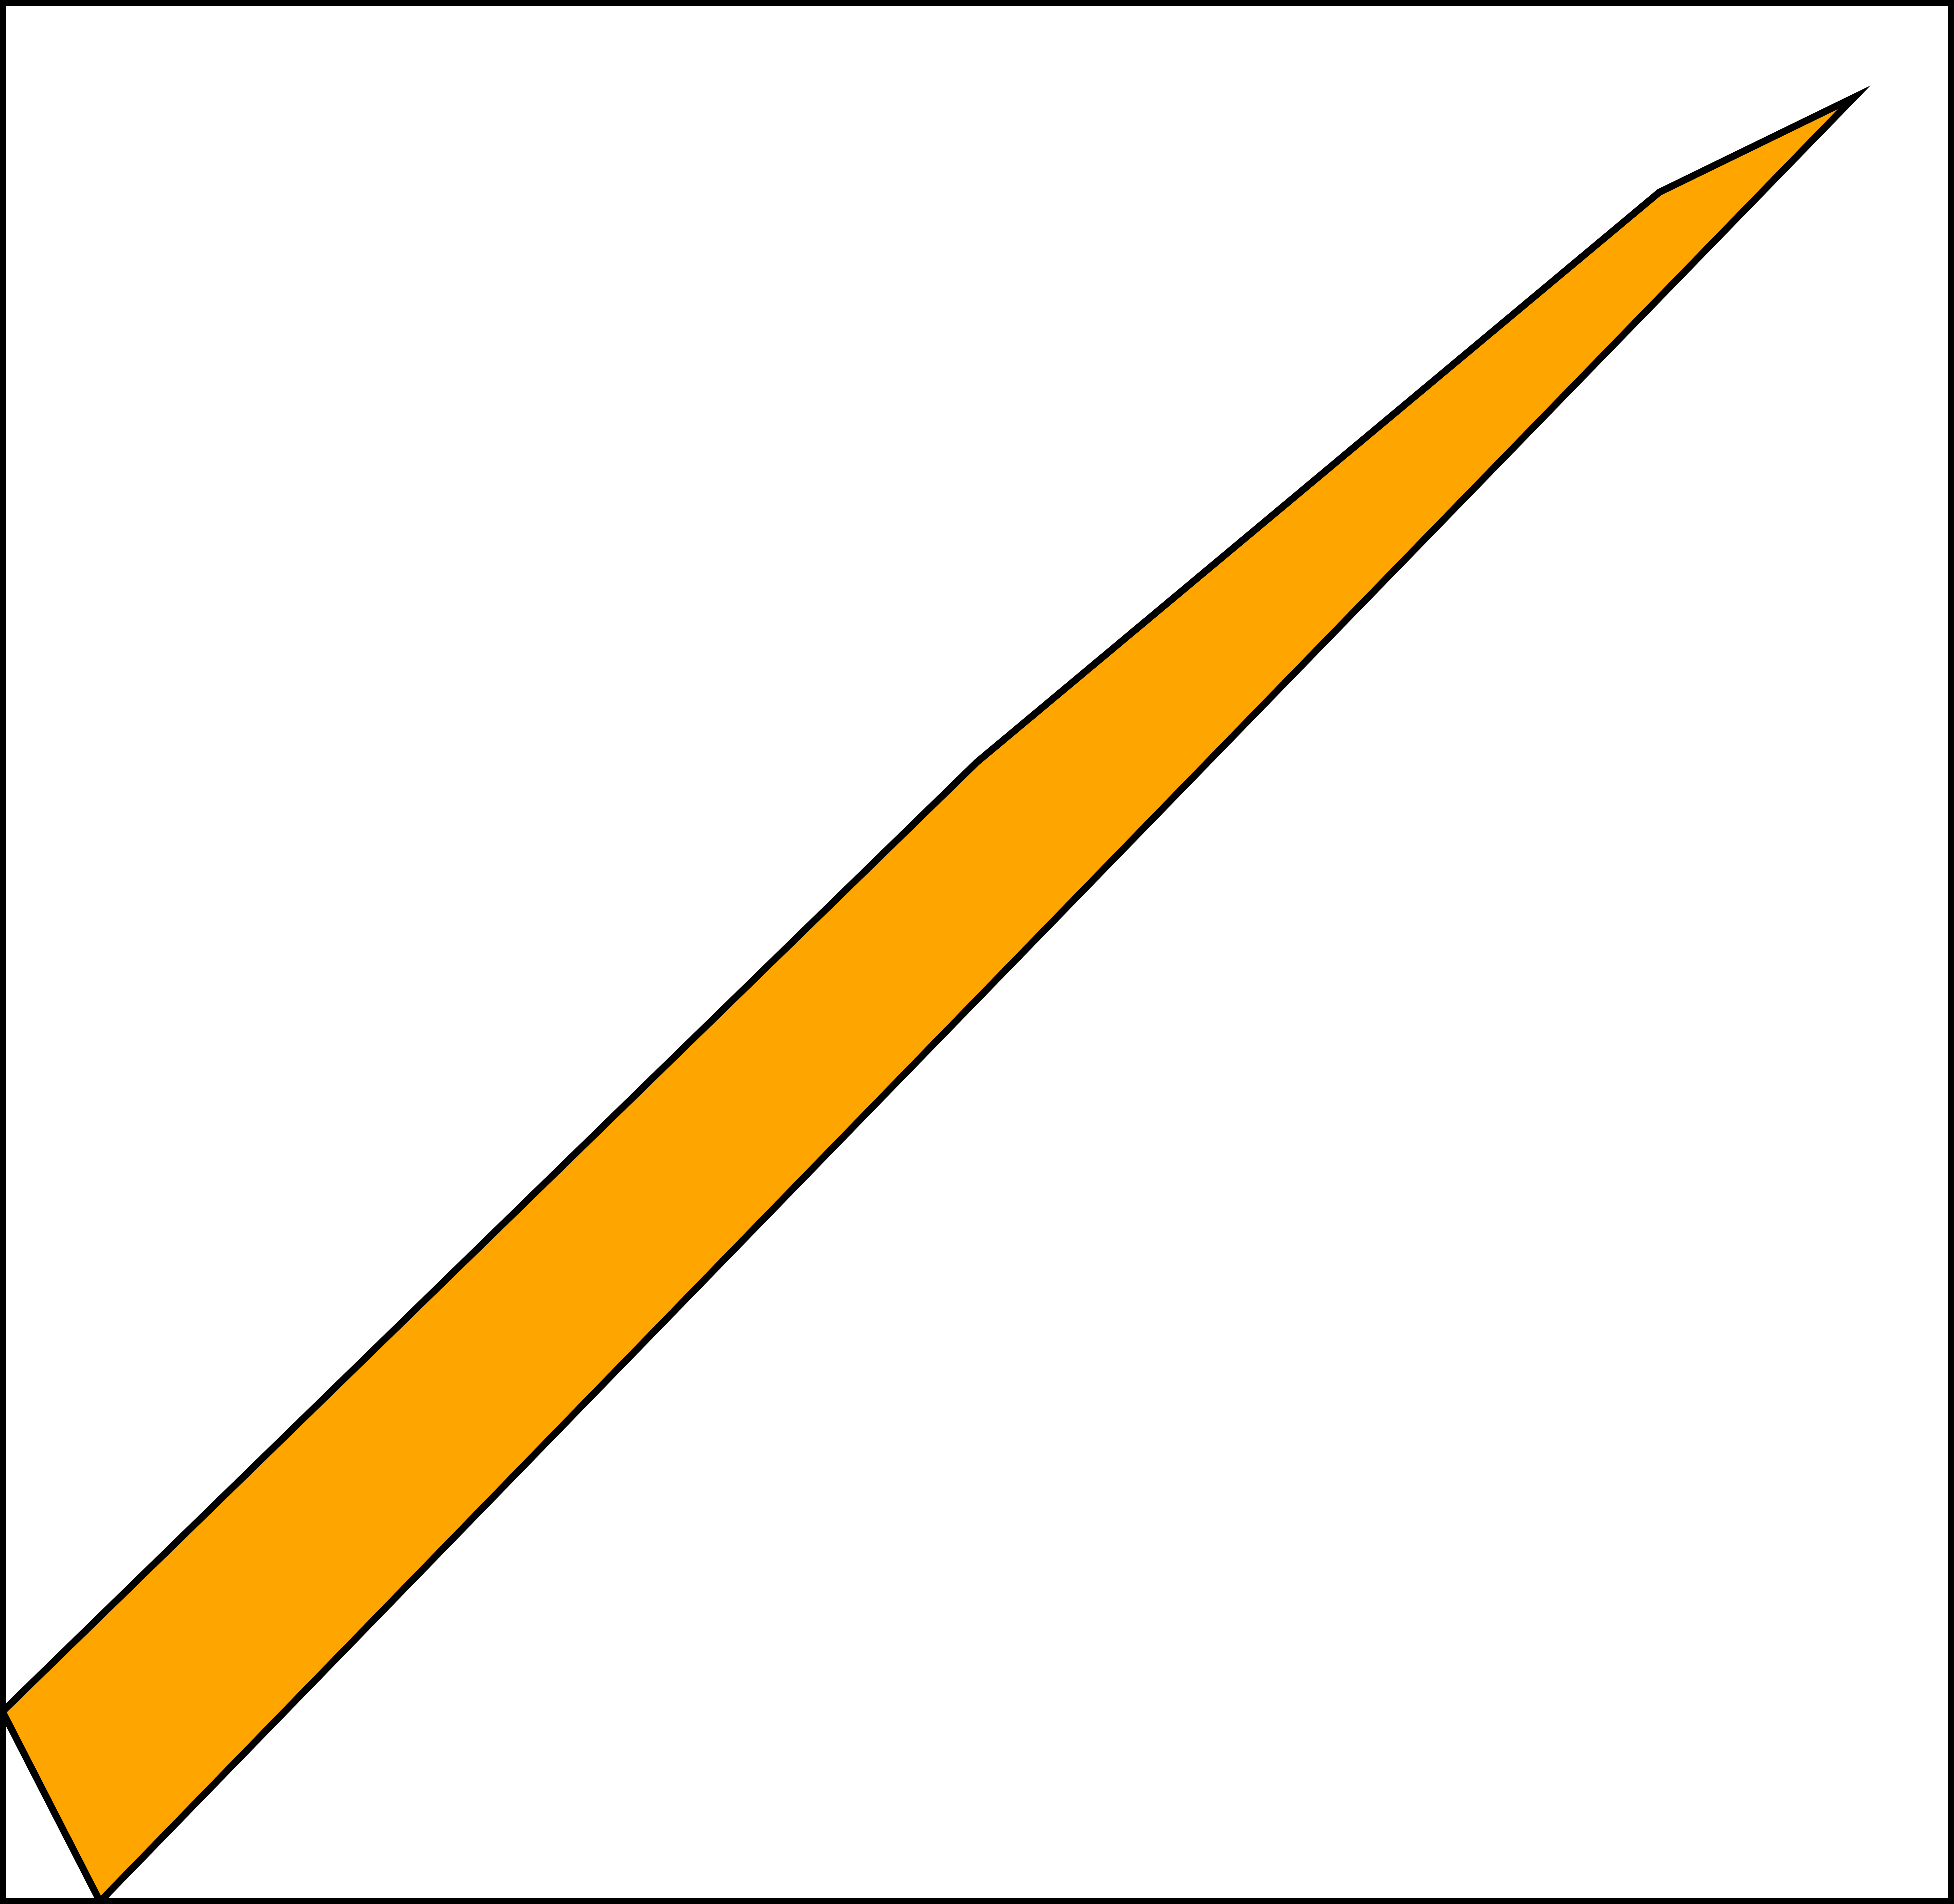
\includegraphics[width=.5\linewidth]{Images/2023_03_07_problematic_polygon.png}
  \caption{A ``problematic'' polygon for \textsc{Polygon Bin Packing}, which is both high and wide but has only small area.}
  \label{image_problematic_polygon}
\end{figure}

\begin{proof}
Throughout the proof we split $I$ into a constant number of sub-instances $I=\bigsqcup_i I_i$ and consider such sub-instances separately. We use without further notice that it is sufficient to show that is possible to pack each sub-instance $I_i$ into at most $\mathcal{O}(\frac{1}{\delta})\opt(I)$ bins in order to obtain an overall packing for $I$ into at most $\mathcal{O}(\frac{1}{\delta})\opt(I)$ bins.

Without loss of generality, we can assume that $\width(p) \leq \height(p)$ for all $p \in I$. All $p \in I$ with $\width(p) > \height(p)$ can be packed analogously after rotation by $\pi/2$ and the packings into unit bins can in the end be rotated back. Note that making this assumption in particular implies that $\width(p) \leq 1-\delta$ for all $p\in I$.

All polygons with $\width(p) \leq \frac{1}{2}$ can be packed with Theorem \ref{polygon_bin_packing_1/M}. So we can assume that $\width(p) \geq \frac{1}{2}$ for all $p \in I$.

Finally, we can also assume that $\area(p) < \frac{\delta}{4}$ for all $p \in I$. Indeed, all polygons $p$ with $\area(p) \geq \frac{\delta}{4}$ can be packed one by one into separate bins which needs no more than $\mathcal{O}(\frac{1}{\delta})$ bins.

Let $I_Q$ be the input consisting of $x$-parallelograms constructed from $I$ with Lemma \ref{polygon_into_parallelogram}. Assume that all of them are tilted to the right and pack those that are not tilted to the right analogously. Note that for each $q \in I_Q$,
\[
\base(q) = \frac{\area(q)}{\height(q)} \leq \frac{2\area(p)}{\height(p)} \leq \delta,
\]
where we used that $\area(p) \leq \frac{\delta}{4}$ and $\height(p)\geq \frac{1}{2}$.
Let $I_R \in \rectangles$ be the instance that for each $q \in I_Q$ contains a rectangle $r=(\base(q),\height(q))$. We now pack $I_R$ with NFDH into a strip of width $\delta$. Such strip has height at most $2 \area(I_R)/\delta + h_{\max}$ by Theorem \ref{nfdh}. Hence, using NF, we can distribute the shelves from this packing, which needs at most $4 \area(I_R)/\delta + 3$ bins of width $\delta$ and height $1$ to pack the rectangles into.

After ordering the parallelograms corresponding to a shelf in the packing of the rectangles by their angle, they can be packed into a shelf of width $1$.

Therefore, $I_Q$ can be packed into
\[
\frac{4 \area(I_R)}{\delta}+3 \leq \frac{8 \area(I)}{\delta}+3
\]
unit bins. Hence, the described method packs $I$ into at most
\[
\frac{8}{\delta}\opt(I) + 3 \leq \bigg (\frac{8}{\delta} + 3 \bigg ) \opt(I)
\]
bins.
\end{proof}

\subsection{An Efficient $\mathcal{O}(C)$-Approximation for \textsc{Polygon Bin Packing} when each Polygon has a Spine from a Set of Constant Size $C$}
\label{section_polygon_same_spine}

In this section, we show that it is possible to pack an instance $I \in \polygons$, for which all polygons $p \in I$ have a spine $s$ from a set $S$ of constant size $C \in \N$, efficiently into at most $\mathcal{O}(C) \opt(I)$ bins efficiently.

First, we need to introduce some notation.

\begin{definition}
Let $p \subset [0,1]^2$ be a polygon. We define
\[
\eta(p) := \max\{\width([x_1,x_2] \times \{y\}) \, | \, [x_1,x_2] \times \{y\} \subset p \}.
\]
If there is a spine $s$ fixed for $p$, we denote by $p^1$ the part of $p$ that lies on the left of $s$ and by $p^2$ the part of $p$ that lies on the right of $s$. In this case, we also set
\[
\eta_1(p) := \eta(p^1) \quad \text{and} \quad \eta_2(p) := \eta(p^2).
\]
\end{definition}

Note that $\max\{\eta_1(p),\eta_2(p)\} \leq \eta(p) \leq \eta_1(p)+\eta_2(p)$ for every polygon $p \in \polygons$.

We prove the following result.

\begin{theorem}
\label{thm_equal_spine}
There is an efficient $\mathcal{O}(1)$-approximation algorithm for \textsc{Polygon Bin Packing} for instances $I \in \polygons$ with the property that all polygons share a spine $s$ (up to translation) with height $H = \height(s) \geq \frac{3}{4}$.
\end{theorem}

\begin{remark}
The factor $\frac{3}{4}$ in the statement is chosen arbitrarily in $(\frac{2}{3},1]$ and only affects the exact approximation ratio. When the factor approaches $\frac{2}{3}$, the approximation guarantee approaches $\infty$.
\end{remark}

\begin{proof}
We assume that $s$ is tilted to the right. As the polygons share a spine $s$, they all have the same height $H$.

Throughout the proof, we write  $M_y:=[0,1] \times \{y\}$ for $y \in [0,1]$. Furthermore, fix some translation $\phi_L \in \Phi$ so that $s_L := \phi_L(s)$ is in the upper left corner of the bin (so that it touches the top and the left side of the bin). Similarly, fix a translation $\phi_R \in \Phi$ so that $s_R := \phi_R(s)$ is in the lower right corner of the bin (so that it touches the bottom and the right side of the bin). We define $x_{\min}$ as the $x$-coordinate of the intersection point of $s_L$ with $M_{1/2}$. Similarly, we define $x_{\max}$ as the $x$-coordinate of the intersection point of $s_R$ with $M_{1/2}$. The two numbers can be explicitly calculated to be $x_{\min} = (1- \frac{1}{2H})\width(s)$ and $x_{\max} = 1-(1- \frac{1}{2H})\width(s)$.

The idea is to give a structural result of an optimal multi-packing $\mathcal{P}_{\opt}$ of the problem. We will then construct a multi-packing, which, using this structural result, can be shown to use at most $\mathcal{O}(1)\opt(I)$ bins.

Let $P$ be an arbitrary packing of a subset $I' \subset I$ into a unit bin. We write $N := \lvert I' \rvert$. Note that since $H > \frac{1}{2}$, all polygons in the packing have their spine crossing $M_{1/2}$ at an $x$-coordinate in $[x_{\min},x_{\max}]$. Let $x_1, \dots, x_{N}$ be the $x$-coordinates of those intersection points in increasing order and denote by $p_1, \dots, p_N$ the affiliated polygons.

\begin{claim}
For all $j \in [N-1]$, it holds that $x_{j+1}-x_j \geq \frac{3H-2}{2(2H-1)}(\eta_2(p_j) + \eta_1(p_{j+1}))$.
\end{claim}

\begin{proof}
Fix some $j \in [N-1]$ and note that $\max\{\eta_2(p_j),\eta_1(p_{j+1})\} \geq \frac{1}{2}(\eta_2(p_j) + \eta_1(p_{j+1}))$. Hence it suffices to show that $x_{j+1}-x_j \geq \frac{3H-2}{2H-1} \max\{\eta_2(p_j),\eta_1(p_{j+1})\}$.

Assume that $\eta_2(p_j) \geq \eta_1(p_{j+1})$. The argument in the other case is analogous. Choose $y \in [0,1]$ so that $\width(P(p^2_j) \cap M_y) = \eta_2(p_j)$ and denote the right-most point in the line $P(p^2_j) \cap M_y$ by $z$. We note that since both $p_j$ and $p_{j+1}$ have height $H$, it surely holds that the distance between $y$ and $\pi_y(P(p_{j+1}))$, which we denote by $\dist(y, \pi_y(P(p_{j+1})))$, is bounded by $1-H$. If $\dist( y, \pi_y(P(p_{j+1}))) = 0$, then surely $x_{j+1}-x_j \geq \width(P(p^2_j) \cap M_y) = \eta_2(p_j)$.
\begin{figure}[h]
\centering
  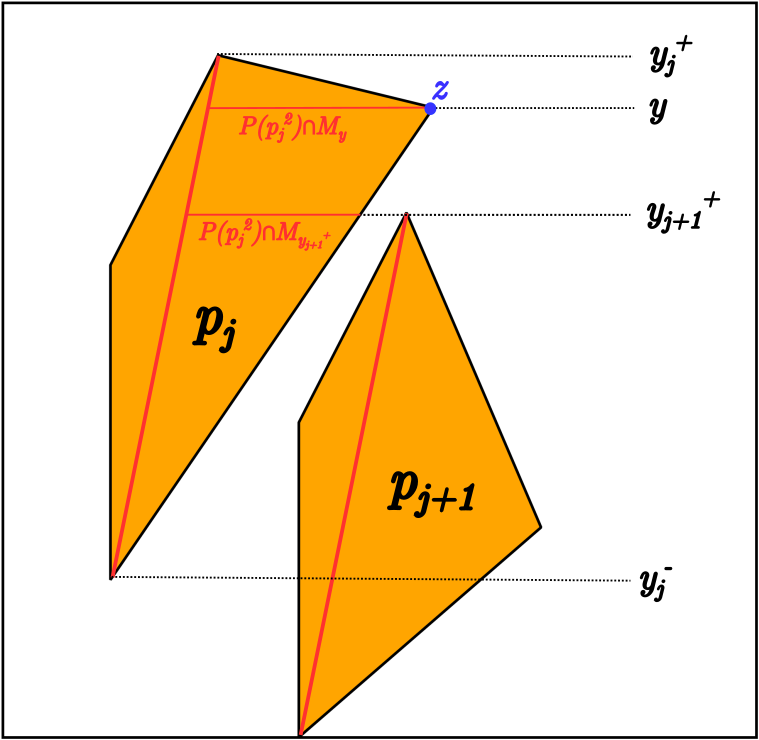
\includegraphics[width=.5\linewidth]{Images/claim_polygons_eqspine3.png}
  \caption{A schematic of the proof of $x_{j+1}-x_j \geq \frac{3H-2}{2(2H-1)}(\eta_2(p_j) + \eta_1(p_{j+1}))$.}
  \label{im_claim_polygon_eqspine}
\end{figure}

So assume that $\dist(y, \pi_y(P(p_{j+1}))) > 0$ and hence $y$ is either above or below $\pi_y(P(p_{j+1}))$. Without loss of generality, assume that it is below and therefore $y_{j+1}^+ := \max \{y' \in \pi_y(P(p_{j+1}))\} < y$ (see Figure \ref{im_claim_polygon_eqspine}). Due to convexity of $P(p_j)$, the line connecting the lower end of the spine of $P(p_j)$ (which is say at height $y_j^- \in [0,1]$) with the point $z$ lies inside of $P(p_j)$. This implies that
\begin{equation}
\label{claim_eq_1}
\width(P(p_j^2) \cap M_{y_{j+1}^+}) \geq \frac{y_{j+1}^+ - y_j^-}{y-y_j^-} \eta_2(p_j).
\end{equation}
Furthermore, since $y_j^- \leq y_{j+1}^+ < y \leq y_j^+ := \max\{y' \in \pi_y(P(p_{j}))\}$, it holds that
\begin{equation}
\label{claim_eq_2}
x_{j+1}-x_j \geq \width(P(p^2_j) \cap M_{y_{j+1}^+}).
\end{equation}
Hence, using
\[
y-y_j^- \geq y_{j+1}^+ - y_j^- = 1-\underbrace{(1-y_{j+1}^+)}_{\leq 1-H}-\underbrace{y_j^-}_{\leq 1-H} \geq 2H-1,
\]
as well as (\ref{claim_eq_1}) and (\ref{claim_eq_2}), we find that
\begin{align*}
x_{j+1}-x_j &\geq \width(P(p^2_j) \cap M_{y_{j+1}^+}) \\
&\geq \frac{y_{j+1}^+ - y_j^-}{y-y_j^-} \eta_2(p_j) \\
&= \frac{y-y_j^- -(y-y_{j+1}^+)}{y-y_j^-} \eta_2(p_j) \\
&\geq \frac{y-y_j^- -(1-H)}{y-y_j^-} \eta_2(p_j) \\
&\geq \frac{3H-2}{2H-1} \eta_2(p_j),
\end{align*}
where in the last inequality, we used that $y-y_j^- \leq y_j^+ - y_j^- \leq 1-H$. This shows the claim.
\end{proof}

From the claim it follows that
\begin{align*}
x_{\max}-x_{\min} &\geq x_N-x_1 \\
& \geq \sum_{j=1}^{N-1} (x_{j+1}-x_j) \\
& \geq \frac{3H-2}{2(2H-1)} \bigg(\sum_{j=2}^{N-1} (\eta_1(p_j) + \eta_2(p_j)) + (\eta_2(p_1) + \eta_1(p_N))\bigg) \\
& \geq \frac{3H-2}{2(2H-1)}\sum_{j=2}^{N-1} \eta(p_j) + \frac{3H-2}{2(2H-1)} (\eta_2(p_1) + \eta_1(p_N)) \\
& \geq \frac{3H-2}{2(2H-1)}\sum_{j=2}^{N-1} \eta(p_j).
\end{align*}

Now, consider an optimal multi-packing $\mathcal{P}_{\opt}=\{P_i\}_{i=1}^{\opt(I)}$ and take out the first and the last polygon (with respect to the ordering coming from $M_{1/2}$) in each bin. If there is only $1$ polygon in a bin, only take out that instead. Denote the polygons that did not get removed this way by $\overline{I} \subset I$.  We pack the removed polygons $I \backslash \overline{I}$ into $1$ bin each, which leads to a multi-packing $\overline{\mathcal{P}}=\{\overline{P}_i\}_{i=1}^{3 \opt(I)}$,where we note that some of the packings might be empty. By what we have discussed before, this packing has the property that for $i \in [\opt(I)]$, it holds that
\begin{equation}
\label{eq_upper_bounding_polygons}
x_{\max}-x_{\min} \geq \frac{3H-2}{2(2H-1)}\sum_{p \text{ is a polygon in the packing } \overline{P_i}} \eta(p)
\end{equation}
and all other packings pack at most $1$ item each. Note that $\overline{I} \subset I$ is exactly the set of polygons packed by any $\overline{P_i}$, for which $i \in [\opt(I)]$.

The idea now is to make a guess $g$ for $\lvert I \backslash \overline{I} \rvert$, remove $g$ items with high $\eta$-value and to then compute a packing for the remaining polygons into not much more than $g$ bins.

Note that surely $\lvert I \backslash \overline{I} \rvert \leq n := \lvert I \rvert$. For $g=1, \dots, n$, take out the $g$ polygons $p \in I$ with highest values $\eta(p)$ and denote the obtained instance by $I_g$.

The idea now is to partition $I_g = \bigsqcup_{k=1}^{K_g} I_{g,k}$ into as few sets as possible in such a way that for each $k \in [K_g]$, it holds that
\begin{equation}
    \label{eq_what_partition_should_do}
    x_{\max}-x_{\min} \geq 2 \sum_{p \in I_{g,k}} \eta(p),
\end{equation}
or $I_{g,k}$ contains only $1$ polygon $p$. Polygons in some $I_{g,k}$ can be packed into a single bin as follows.

Fix some $k \in \N$ and say $I_{g,k}$ consists of polygons $p_1, \dots, p_{N_{g,k}}$. If $N_{g,k}=1$, then we can clearly pack $I_{g,k}$ into a unit bin. So assume that $N_{g,k} > 1$. We construct a packing $P_{g,k}$ of $I_{g,k}$ into a strip $[0,\infty) \times [0,1]$ as follows. Place polygon $p_1$ so that it touches the left and the upper boundary of the strip. Then place polygon $p_2$ below it so that it touches the left boundary of the strip, as well as $p_1$. Further polygons $p_3, p_4, \dots$ are now being placed so that a new placed polygon always touches the left boundary of the strip and the last placed polygon. Repeat this process until there is not enough space due to the bottom of the strip anymore. We do now place a next polygon so that it touches the the last placed polygon and the bottom of the strip instead. The remaining polygons are now being placed so that a newly placed polygon always touches the bottom boundary of the strip and the last placed polygon. Note that the fact that all polygons have the same height $H$ ensures that the procedure works, and no polygon touches another one except for the one placed directly before and after it. In the following, we show that $\width(P_{g,k}) \leq 1$ and that hence $P_{g,k}$ fits into a unit bin.

To see this, write $x_1, \dots, x_{N_{g,k}}$ for the $x$-coordinates of the intersection points of the spines of $p_1, \dots, p_{N_{g,k}}$ in $P_{g,k}$ with $M_{1/2}$. First, consider $p_1$. Note that $P_{g,k}(p_1)$ necessarily intersects with $s_L$ (which we recall is the placement of the spine $s$ so that it is in the upper left corner). This is because $P_{g,k}(p_1)$ touches the left boundary, contains a copy of this spine and has its lower end at the same height as the lower end of $s_L$. Thus, if $y_1 \in [1-H,1]$ is any height at which such intersection happens, we denote by $t$ the segment at height $y_1$ that is parallel to the $x$-axis, starts on $s_L$ and ends at the spine of the placement of $p_1$. We find that
\[
x_1 - x_{\min}(I) = \width(t) \leq \eta_1(p_1) \leq \eta(p_1).
\]

Now let $j \in [N_{g,k}-1]$ and consider $p_j$ and $p_{j+1}$. Then they touch somewhere in $P_{g,k}$, say at height $y_j \in [0,1]$. Therefore
\begin{align*}
x_{j+1} - x_j &\leq \width((p^2_j \cup p^1_{j+1}) \cap M_{y_j}) \leq \eta_2(p_j) + \eta_1(p_{j+1}) \leq \eta(p_j) + \eta(p_{j+1}).
\end{align*}

Writing $x_0 := x_{\min}$ and using (\ref{eq_what_partition_should_do}), we hence find that
\[
x_{N_{g,k}} = \sum_{j=0}^{N_{g,k}-1} (x_{j+1} - x_j) \leq 2 \sum_{p \in I_{g,k}} \eta(p) + x_{\min}(I) - \eta(p_{N_{g,k}})  \leq x_{\max}(I) - \eta(p_{N_{g,k}}).
\]
We finally consider $p_{N_{g,k}}$. Note that since $p_{N_{g,k}}$ is placed on the bottom of the strip, its spine in $P_{g,k}$ can at most extend horizontally to the right until $x_{N_{g,k}} + (1-\frac{1}{2H})\width{s}$ (that is, the upper end of the spine of $p_{N_{g,k}}$ has such $x$-coordinate). But this is exactly equal to $x_{N_{g,k}} + (1-x_{\max}(I))$. In particular,
\[
\width(P_{g,k}) \leq x_{N_{g,k}} + (1-x_{\max}(I)) + \eta_2(p_{N_{g,k}}) \leq 1 + x_{N_{g,k}} -(x_{\max}(I) - \eta(p_{N_{g,k}})) \leq 1,
\]
which shows that $I_{g,k}$ can be packed by $P_{g,k}$ into a unit bin.

So it suffices to find a partition $I_g = \bigsqcup_{k=1}^{K_g} I_{g,k}$ satisfying (\ref{eq_what_partition_should_do}) for $g \in [2n]$ and show that there is $g$ so that $K_g + g$ is not much bigger than $\opt(I)$. 

We first show the following claim.

\begin{claim}
Let $I_{BP}$ be an instance for $(1D)$-\textsc{Bin Packing} and let $\alpha \geq 1$. Define $\overline{I_{BP}} := \{\overline{s}\}_{s \in I_{BP}}$, where for $s \in I_{BP}$,  we set $\overline{s}:=\min\{\alpha s,1\}$. Then
\[
\opt_{BP}(\overline{I_{BP}}) \leq (2 \alpha+1) \opt_{BP}(I_{BP}),
\]
where $opt_{BP}$ is the function that assigns to an instance of \textsc{Bin Packing} its optimal solution.
\end{claim}
\begin{proof}
Consider the partition $I_{BP}=\bigsqcup_{j=1}^l A_j$ corresponding to an optimal solution. Then $\sum_{s \in A_j} s \leq 1$ and hence, writing $\overline{A_j} = \{\overline{s}\}_{s \in A_j}$, it holds that $\sum_{\overline{s} \in \overline{A_j}} \overline{s} \leq \alpha$. With \textsc{NextFitDecreasing}, we can hence pack $\overline{A_j}$ into at most $2 \alpha + 1$ bins . Doing this for all $j \in [l]$, we obtain a feasible solution of \textsc{Bin Packing} for the instance $\overline{I_{BP}}$ into at most $(2\alpha + 1) l = (2 \alpha + 1) \opt_{BP}(I_{BP})$ bins.
\end{proof}

For $p \in I_g$, we write $\rho(p):=\min \{2\eta(p),x_{\max}-x_{\min}\}$. Use FFDH to find a $\frac{3}{2}$-approximation to \textsc{Bin Packing} efficiently (see~\cite{SimchiLevi1994NewWR}) for the instance $\{\rho(p)\}_{p \in I_g}$ but for bins of size $x_{\max}-x_{\min}$. Denote the number of bins this solution needs by $K_g$ and partition $I_g$ according to this solution into sets $I_g = \bigsqcup_{k=1}^{K_g} I_{g,k}$. Note that the partition satisfies exactly the property (\ref{eq_what_partition_should_do}).

Denote the optimal solution of an instance $J$ for \textsc{Bin Packing} for bins of size $x_{\max}-x_{\min}$ by $\opt_{BP^s}(J)$. We now consider how big the value of $K_g$ is in the case when $g=\lvert I \backslash \overline{I} \rvert$. In this case, using the last claim for $\alpha := 2/\big(\frac{3H-2}{2(2H-1)}\big) = \frac{4(2H-1)}{3H-2}$ and recalling that $I_g$ is obtained from $I$ after taking out the $g$ polygons $p$ with biggest values of $\eta(p)$, we find that
\begin{align*}
K_{\lvert I \backslash \overline{I} \rvert} & \leq \frac{3}{2}\opt_{BP^s}(\{\rho(p)\}_{p \in I_{\lvert I \backslash \overline{I} \rvert}}) \\
&\leq \frac{3}{2}\opt_{BP^s}(\{\rho(p))\}_{p \in \overline{I}}) \\ 
&\leq \frac{3}{2} \bigg(\frac{8(2H-1)}{3H-2}+1 \bigg) \opt_{BP^s} \bigg( \Big\{\frac{3H-2}{2(2H-1)} \eta(p) \Big\}_{p \in \overline{I}}\bigg) \\
&\leq \frac{3}{2} \bigg(\frac{8(2H-1)}{3H-2}+1 \bigg) \opt(I) \\
&= \bigg(\frac{24H-12}{3H-2} + \frac{3}{2}\bigg) \opt(I),
\end{align*}
where the last inequality follows from (\ref{eq_upper_bounding_polygons}).

So take the value of $g \in [n]$ for which $g+K_g$ is minimized. Then, recalling that $\lvert I \backslash \overline{I} \rvert \leq 2 \opt(I)$, it holds that
\[
g+K_g \leq \lvert I \backslash \overline{I} \rvert + K_{\lvert I \backslash \overline{I} \rvert} \leq \bigg(\frac{7}{2} + \frac{24H-12}{3H-2}\bigg) \opt(I) \leq 27.5 \opt(I),
\]
using that $H \geq \frac{3}{4}$. This concludes the proof.
\end{proof}

\begin{remark}
A next goal could be to show the existence of an efficient $\mathcal{O}(1)$-approximation for instances $I \in \polygons$ for which there is an angle $\alpha \in [0, \pi]$ so that each polygon $p \in I$ has a spine $s_p$ with angle $\alpha$.
\end{remark}

We conclude the section with the following corollary.

\begin{corollary}
Let $C \in \N$. There is an efficient $\mathcal{O}(C)$-approximation algorithm for \textsc{Polygon Bin Packing} for instances $I \subset \polygons$ satisfying the following. There is a set $S$ of lines in $[0,1]^2$, so that $\lvert S \rvert \leq C$ and with the property that each polygon $p \in I$ has a spine $s$ in the set $S$ (up to translation).
\end{corollary}

\begin{proof}
First, we note that all polygons with height smaller than $\frac{3}{4}$ can easily be packed using Theorem \ref{polygon_bin_packing_1_minus_delta} for $\delta = \frac{1}{4}$. This needs at most $\mathcal{O}(1) \opt(I)$ bins. We call the remaining set of polygons $\overline{I}$. Partition $\overline{I}:=\bigsqcup_{s \in S} I_s$ so that for all $s \in S$, all $p \in I_s$ have a spine that (up to a translation) is equal to $s$. Packing each $I_s$, $s \in S$, separately with the algorithm from Theorem \ref{thm_equal_spine}, we need at most $C\mathcal{O}(1)\opt(\overline{I}) \leq \mathcal{O}(C)\opt(I)$ bins.
\end{proof}


\bibliography{ref_MT.bib}


\end{document}
